\documentclass[english,12pt,a4paper,pdftex]{article}

%% Nämä komennot asettavat oikean tekstiencodauksen.
\usepackage[utf8]{inputenc}
\usepackage[OT1]{fontenc}

\usepackage{natbib}

\bibpunct{(}{)}{;}{a}{,}{,}

\usepackage{verbatim}
\usepackage{multirow}

%% Tämä paketti on pakollinen
%% Valitse korkeakoulusi näistä: arts, biz, chem, elec, eng, sci.
%%
%% This package is required
%% Choose your school from arts, biz, chem, elec, eng, sci.
\usepackage[sci]{aaltothesis}

%% Jos käytät latex-komentoa käännettäessä (oletusarvo) 
%% kuvat kannattaa tehdä eps-muotoon. Älä käytä ps-muotoisia kuvia!
%% Käytä seuraavaa latex-komennon ja eps-kuvien kanssa 
%%
%% Jos tääs käytät pdflatex-komentoa, joka kääntää tekstin suoraan
%% pdf-tiedostoksi, kuvasi on oltava jpg-formaatissa tai pdf-formaatissa.
%%
%% Use this if you run pdflatex and use jpg/pdf-format pictures.
%%
\usepackage{graphicx}

%% Saat pdf-tiedoston viittaukset ja linkit kuntoon seuraavalla paketilla.
%% Paketti toimii erityisen hyvin pdflatexin kanssa. 
%%
%% Use this if you want to get links and nice output with pdflatex
\usepackage[pdfpagemode=None,colorlinks=false,urlcolor=red,linkcolor=blue,citecolor=black,pdfstartview=FitH]{hyperref}


%% Jos et jostain syystä tykkää käyttää
%% edellistä hyperref pakettia, voit käyttää myös seuraavaa pakettia
%% (tarvitaan lähinnä url-komennon määrittämiseen ja formatoimiseen)
%%
%% Use this if you do not like hyperref package - this
%% defines url environment and formats it correctly
\usepackage{url}

%% Matematiikan fontteja, symboleja ja muotoiluja lisää, näitä tarvitaan usein 
%%
%% Use this if you write hard core mathematics, these are usually needed
% \usepackage{amsfonts,amssymb,amsbsy}  

%% Vaakasuunnan mitat, ÄLÄ KOSKE!
\setlength{\hoffset}{-1in}
\setlength{\oddsidemargin}{35mm}
\setlength{\evensidemargin}{25mm}
\setlength{\textwidth}{15cm}
%% Pystysuunnan mitat, ÄLÄ KOSKE!
\setlength{\voffset}{-1in}
\setlength{\headsep}{7mm}
\setlength{\headheight}{1em}
\setlength{\topmargin}{25mm-\headheight-\headsep}
\setlength{\textheight}{23cm}


%% Kaikki mikä paperille tulostuu, on tämän jälkeen
%%
%% Output starts here
\begin{document}

%% Korjaa vastaamaan korkeakouluasi, jos automaattisesti asetettu nimi on 
%% virheellinen 
%%
%% Change the school field to describe your school if the autimatically 
%% set name is wrong
% \university{aalto University}{aalto-Yliopisto}
% \school{School of Electrical Engineering}{SähköTekniikan korkeakoulu}

%% Vain kandityölle: Korjaa seuraavat vastaamaan koulutusohjelmaasi
%%
%% Only for B.Sc. thesis: Choose your degree programme. 
% \degreeprogram{Electronics and electrical engineering}% {Elektroniikka ja sähkötekniikka}
%%

%% Vain DI/M.Sc.- ja lisensiaatintyölle: valitse laitos, 
%% professuuri ja sen professuurikoodi. 
%%
%% Only for M.Sc. and Licentiate thesis: Choose your department,
%% professorship and professorship code. 
\department{Department of Media Technology}
{Mediatekniikan laitos}
\professorship{Media Technology}{Mediatekniikka}
\code{T-111}
%%

%% Valitse yksi näistä kolmesta
%%
%% Choose one of these:
%\univdegree{BSc}
\univdegree{MSc}
%\univdegree{Lic}

%% Oma nimi
%%
%% Should be self explanatory...
\author{Mikko Koski}

%% Opinnäytteen otsikko tulee vain tähän. Älä tavuta otsikkoa ja
%% vältä liian pitkää otsikkotekstiä. Jos latex ryhmittelee otsikon
%% huonosti, voit joutua pakottamaan rivinvaihdon \\ kontrollimerkillä.
%% Muista että otsikkoja ei tavuteta! 
%% Jos otsikossa on ja-sana, se ei jää rivin viimeiseksi sanaksi 
%% vaan aloittaa uuden rivin.
%% 
%% Your thesis title. If the title is very long and the latex 
%% does unsatisfactory job of breaking the lines, you will have to
%% break the lines yourself with \\ control character. 
%% Do not hyphenate titles.
\thesistitle{Effective communication media for customer feedback in agile software projects}{Tehokkaat kommunikaatiokanavat asiakaspalautteen antamiseen ketterissä ohjelmistoprojekteissa}

\place{Espoo}
%% Kandidaatintyön päivämäärä on sen esityspäivämäärä! 
%% 
%% For B.Sc. thesis use the date when you present your thesis. 
\date{20.3.2012}

%% Kandidaattiseminaarin vastuuopettaja tai diplomityön valvoja.
%% Huomaa tittelissä "\" -merkki pisteen jälkeen, 
%% ennen välilyöntiä ja seuraavaa merkkijonoa. 
%% Näin tehdään, koska kyseessä ei ole lauseen loppu, jonka jälkeen tulee 
%% hieman pidempi väli vaan halutaan tavallinen väli.
%%
%% B.Sc. or M.Sc. thesis supervisor 
%% Note the "\" after the comma. This forces the following space to be 
%% a normal interword space, not the space that starts a new sentence. 
\supervisor{Prof.\ Tapio Takala}{Prof.\ Tapio Takala}

%% Kandidaatintyön ohjaaja(t) tai diplomityön ohjaaja(t)
%% 
%% B.Sc. or M.Sc. thesis advisors(s). 
%%
%% Note that there has been a change in the official EN translation
%% of the Finnish title ``ohjaaja'' which in the previous version (1.5) 
%% of this document was called ``instructor''. The recommended
%% translation is now ``advisor''.  
%% However, the LaTeX internal variable remains \instructor
%% as there is little point to change the variable name. 
%%
%\instructor{Prof. Pirjo Professori}{Prof. Pirjo Professori}
\instructor{Risto Sarvas}{Risto Sarvas}
%\instructor{M.Sc.\ (Tech.) Polli Pohjaaja}{DI Polli Pohjaaja}

%% Aaltologo: syntaksi:
%% \uselogo{aaltoRed|aaltoBlue|aaltoYellow|aaltoGray|aaltoGrayScale}{?|!|''}
%% Logon kieli on sama kuin dokumentin kieli
%%
%% Aalto logo: syntax:
% \uselogo{aaltoRed|aaltoBlue|aaltoYellow|aaltoGray|aaltoGrayScale}{?|!|''}
%% Logo language is set to be the same as the document language.
\uselogo{aaltoRed}{''}

%% Tehdään kansilehti
%%
%% Create the coverpage
\makecoverpage


%% Suomenkielinen tiivistelmä
%% 
%% Finnish abstract
%%
%% Tiivistelmän avainsanat
\keywords{kommunikaatio, ketterä ohjelmistotuotanto, asiakaspalaute}
%% Tiivistelmän tekstiosa
\begin{abstractpage}[finnish]
  Tiivistelmässä on lyhyt selvitys (noin 100 sanaa)
  kirjoituksen tärkeimmästä sisällöstä: mitä ja miten on tutkittu,
  sekä mitä tuloksia on saatu. 
  Tiivistelmässä on lyhyt selvitys (noin 100 sanaa)
  kirjoituksen tärkeimmästä sisällöstä: mitä ja miten on tutkittu,
  sekä mitä tuloksia on saatu. 

  Tiivistelmässä on lyhyt selvitys (noin 100 sanaa)
  kirjoituksen tärkeimmästä sisällöstä: mitä ja miten on tutkittu,
  sekä mitä tuloksia on saatu. 
  Tiivistelmässä on lyhyt selvitys (noin 100 sanaa)
  kirjoituksen tärkeimmästä sisällöstä: mitä ja miten on tutkittu,
  sekä mitä tuloksia on saatu. 
  Tiivistelmässä on lyhyt selvitys (noin 100 sanaa)
  kirjoituksen tärkeimmästä sisällöstä: mitä ja miten on tutkittu,
  sekä mitä tuloksia on saatu. 
\end{abstractpage}

%% Pakotetaan uusi sivu varmuuden vuoksi, jotta 
%% mahdollinen suomenkielinen ja englanninkielinen tiivistelmä
%% eivät tule vahingossakaan samalle sivulle
%%
%% Force new page so that English abstract starts from a new page
\newpage
%
%% English abstract, uncomment if you need one. 
%% 
%% Abstract keywords
\keywords{communication, agile, software, feedback, media}
%% Abstract text
\begin{abstractpage}[english]
 Your abstract in English. Try to keep the abstract short, approximately 
 100 words should be enough. Abstract explains your research topic, 
 the methods you have used, and the results you obtained.  
\end{abstractpage}
%% Note that 
%% if you are writting your master's thesis in English place the English
%% abstract first followed by the possible Finnish abstract

%% Esipuhe 
%%
%% Preface
\mysection{Preface}
TODO: Haluan kiittää Professori Pirjo 
Professoria ja ohjaajaani Olli Ohjaajaa hyvästä ja 
huonosta ohjauksesta.\\

\vspace{5cm}
Otaniemi, 9.3.2012

\vspace{5mm}
{\hfill Mikko Koski \hspace{1cm}}

%% Pakotetaan varmuuden vuoksi esipuheen jälkeinen osa
%% alkamaan uudelta sivulta
%%
%% Force new page after preface
\newpage




%% Sisällysluettelo
%% addcontentsline tekee pdf-tiedostoon viitteen sisällysluetteloa varten
%% 
%% Table of contents. 
%\addcontentsline{toc}{section}{Sisällysluettelo}
\addcontentsline{toc}{section}{Contents}
%% Tehdään sisällysluettelo
%%
%% Create it. 
\tableofcontents


%% Symbolit ja lyhenteet
%%
%% Symbols and abbreviations
% \mysection{Symbolit ja lyhenteet}
% \mysection{Symbols and abbreviations}

% \subsection*{Lyhenteet}

\clearpage

\subsection*{Abbreviations}

\begin{tabular}{ll}
MRT         & Media Richness Theory \\
MST         & Media Synchronocity Theory \\
API         & Application Programming Interface
\end{tabular}


%% Sivulaskurin viilausta opinnäytteen vaatimusten mukaan:
%% Aloitetaan sivunumerointi arabialaisilla numeroilla (ja jätetään
%% leipätekstin ensimmäinen sivu tyhjäksi, 
%% ks. alla \thispagestyle{empty}).
%% Pakotetaan lisäksi ensimmäinen varsinainen tekstisivu alkamaan 
%% uudelta sivulta clearpage-komennolla. 
%% clearpage on melkein samanlainen kuin newpage, mutta 
%% flushaa myös LaTeX:n floatit 
%% 
%% Corrects the page numbering, there is no need to change these
\cleardoublepage

\storeinipagenumber
\pagenumbering{arabic}
\setcounter{page}{1}

\clearpage

%% Leipäteksti alkaa
%%
%% Text body begins. Note that since the text body
%% is mostly in Finnish the majority of comments are
%% also in Finnish after this point. There is no point in explaining
%% Finnish-language specific thesis conventions in English.
\section{Introduction}

Agile software development in its essence is all about feedback. The core principle of agile development is to have short iterations and deliver a possibly shippable product increment after each iteration \citep{schwaber2009agile}. The delivered product increment enables a possibility for customer to give feedback about the outcome of the iteration and this way direct the development organization to the correct route.

Since the rise of agile software development methods, customer communication and customer collaboration have been taken seriosly and they have been identified as one of the key elements in successful software projects \citep{agilemanifesto}. Also, in previous research it has been shown that a lack of communication and customer involvement is one of the biggest challenges faces by agile teams \citep{korkala2006}.

Agile software development principles emphasis on intense customer communication. One of the twelve Agile Manifesto principles states that "the most efficient and effective method of conveying information to and within a development team is face-to-face conversation". \citep{agilemanifesto} As a result, the first version of eXtreme Programming (XP), which is one of the agile software process frameworks demanded an Onsite-customer to support face-to-face communication \citep{wake2002}. However, this requirement has been removed and replaced with a practice called Real Customer Involvement where the customer should be involved weekly \citep{korkala2006}.

Face-to-face communication, even though being effective communication method comes with a requirement to share the same physical location and time slot. However, as \citet{derosa2004} have pointed out organization are relying more heavily on virtual teams due to a more competitive global market, the benefits of integrating the work of specialized employees who might be geographically dispersed and the need to save time and travel expenses. 

The use of virtual teams and the need to maintain customer involvement create a request to research ways how these elements can be combined. The need has been identified in a previous research. \citet{korkala2006} underline that because of the lack of Onsite-customer it is essential that communication and feedback mechanisms should receive special attention in agile development.

A lot of research has been conducted about communication is software projects but not so many with the focus on some specific aspect of communication. I believe that customer communication in software projects is a wide subject that includes different types of communication methods in different situations. For example, the communication required while doing planning is very different from the communication required while customer is giving feedback. Thus, it makes sense to focus on specific area of communication.

\textbf{Introa tässä rakenne: The structure of the thesis is first literature, 4 theories, then prototype and last interviews}

Tämä luku vastaa kysymykseen:

\begin{itemize}
\item What's the research problem, bigger phenomenon
\item Why does the problem matter?
\end{itemize}

%% Ensimmäinen sivu tyhjäksi
%% 
%% Leave first page empty
\thispagestyle{empty}



%% Opinnäytteessä jokainen osa alkaa uudelta sivulta, joten \clearpage
%%
%% In a thesis, every section starts a new page, hence \clearpage

\clearpage

\section{Literature}

Vastataan kysymykseen:

\begin{itemize}
\item What has been studied before?
\item What hasn't been studied yet?
\end{itemize}

\subsection{Definitions}

In this section the most relevant terms and concepts for the thesis are introduces and defined.

\subsubsection{Customer feedback}

\begin{comment}
\begin{itemize}
\item What does \textit{customer} mean?
\item What does \textit{feedback} mean? Feedback from what?
\end{itemize}
\end{comment}

In this thesis \textit{customer} refers to a person in a software project who is the feedback provider. In the context of external software projects customer refers to a representative from the customer organization who gives feedback to the supplier organization. In the context of internal software project customer refers to the representative in the internal organization who is in response of the project outcome and who provides the feedback to the development team.

As the context of the thesis is in agile software development, by customer I refer to Product Owner. Product Owner is a agile team member who is responsible of product outcome. Product Owner maintains the product backlog, scope and prioritizes the items in the backlog. Because Product Owner is the one who is responsible of the project outcome, she is also a person who most likely provides the team with the most valuable feedback \citep{pichler2010}.

\textit{Feedback} is a part of the communication between customer and the software supplier. It is a phase of customer--supplier communication that can happen only after the supplier has delivered something concrete to the customer. Obviously, if supplier has not delivered yet anything, there is very little for customer to give feedback from. Thus, it can be argued, that feedback is a form of communication that happens only after the project has been going on for some time.

Feedback can be given from various subjects in software projects. Feedback can be given for example from the working practices, working processes, design documents, user-interface drafts or working piece of software. In this thesis the main focus is in feedback given about the working piece of software which has been delivered to the customer. There are various ways how software can be delivered from development team to customer (e.g. DVDs, email etc.). However, in agile software projects the preferred way to deliver software to customer to test it is a Continuous Integration or a staging server. \citep{CI lähde} Thus, in this thesis it is assumed that the feedback is given from a software that is running or otherwise available from a testing server which is updated real-time as the development goes on.

\subsubsection{Effective communication}

\begin{comment}
\begin{itemize}
\item What does \textit{effective} mean? 
\item What makes communication efective? 
\item What are the properties (in this paper) that make communication efective
\end{itemize}

Kirjoita tähän, että sosiaaliset hyödyt eivät kuulu tähän kategoriaan. Työssä mitataan vain informaation siirtymistä ja sen tehokkuutta.
\end{comment}

Communication is in essential role in todays agile software development. Intense communication between the customer and the development leads to various benefits. The most important benefit of communication is information and knowledge sharing. However, other benefits are also in a big role in software development. Through communication the customer and the development team can build a trust and team spirit. These aspects are highly valuable in order to increase the motivation of the team and happiness of the customer.

Because the benefits of communication are manifold also the effectiveness of the communication media can ambiguous. While one communication media can be effective in sheer information or knowledge transfer other media can be powerful in building team spirit and bond between customer and the developers.

Even though I recognize the importance of the social aspects of communication and communication media the main scope of this thesis is on more result-oriented properties of communication performance. In this thesis effectiveness of communication media refers to medium's ability to transfer information from an individual to another in order to achieve a mutual understanding. From the feedback point of view this means the ability for the customer to send the feedback message to the developers so that they are able to act accordingly.

This approach to the communication effectiveness was chosen because of two main reasons. First, to make the thesis focused and keep the research scope in hand the social aspects of communication was scoped out. Second, the selected theories, Media Richness, Media Synchronicity, Media Naturalness and Media Fitness support well this approach. However, as mentioned, I recognize the need to investigate also the social aspects of communication and thus it would be valuable subject for further research.

\subsubsection{Agile software projects}

\begin{itemize}
\item What does \textit{agile} mean in this paper?
\end{itemize}

\subsection{Communication in agile software projects}

\begin{itemize}
\item What has been studied about communication?
\item What has been studied about agile software projects?
\item Why hasn't feedback been studied?
\end{itemize}

\subsection{Media theories}

\textbf{Media Fitness Theory} is a rather new and interesting theory. It was developed by \citet{higa2007}. The theory was selected as a port of this thesis because it mainly focuses to the media selection. Media selection is especially important from the point of this thesis. Understanding the reasons why one medium is preferred over another helps to understand what are the properties of a medium that makes it better fit for a communication task in question.

The theory of Media Fitness is another theory that tries to address to the mismatch between the previously formed theories and the empirical evidence of media selection. The theory is influenced by Media Richness by \citet{daft1986} Theory and Social Influence Perspectives by Fulk et al. \textbf{LÄHDE}.

Social Influence theories and social aspects to the effectiveness of communication were are excluded. The reason is two-fold. First, in the name of keeping the scope of the thesis, this research focuses on the properties of communication media, not on the social factors affecting to media selection. Second, the main objective is to support development of new communication media for customer feedback. The new communication media development benefits more from research which concentrates of media properties than the social factors. \textbf{Tää pitää uudelleen kirjottaa koko kappale varmaan}

The theory has been empirically proven to provide rather good match between the teorethical prediction of media selection and the actual choice \citep{higa2007} \citep{gu2011}.

In the following subsection each theory selected to be part of the thesis are described in detail.

Tässä luvussa esitellään teoriat, joiden pohjalta arvioidaan kommunikaatiotyökaluja.

Etsitään vastauksia mm. seuraaviin kysymyksiin:

Perustele miksi "social influence" on tai ei ole otettu huomioon.

Muita hylättyjä: 
- Relatioship development, Walther 1992 (Interpersonal Effects in Computer-Mediated Interaction A Relational Perspective)
- Channel expansion, Carlson and Zmud 1999 (Channel expansion theory and the experiental nature of media richness perceptions)
- Zigur buckland, task-technology fit
- Nunamaker, Dennis, Valacich - Electronic meeting systems to support group work

\begin{itemize}
\item Millaisia ominaisuuksia hyvässä kommunikaatiotyökalussa on?
\item Miten näitä ominaisuuksia pystyttäisiin tuomaan mukaan tietokoneavusteiseen kommunikaatiotyökaluun (vai pystyykö)
\end{itemize}

\subsubsection{Media Richness Theory}

The theory of media richness was proposed by \citet{daft1986}. The theory is well-known and widely supported. However, it has been faces a lot of critisism \citep{dennis1999} \citep{korkala2006}. New theories, such as media synchronicity theory and media naturalness theory have arised to answer the critisism media richness theory has faced.

The main assertion of media richness theory is that different communication methods can be classified either high or low in their "richness" based on their capacity to facilitate shared meaning. In order of decreasing richness, the media classifications are face-to-face, telephone, written personal documents such as letters or memos, impersonal and unaddressed written documents such as fliers or standard formal reports. The hierarchical classification illustrated figure~\ref{fig:hierarchy_of_media_richness}.

\begin{figure}[htb]
\begin{center}
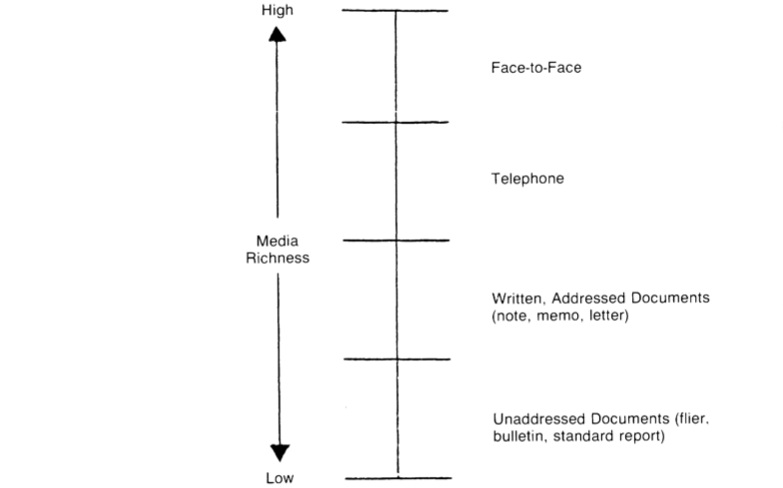
\includegraphics[width=1.0\textwidth]{hierarchy_of_media_richness.png}
\end{center}
\caption{Hierarchy of media richness \citep{daft1987}}
\label{fig:hierarchy_of_media_richness}
\end{figure}

The theory also utilizes a concept of message uncertainty and equivocality. \textbf{Uncertainty} exists if information can be interpreted unambiguously but there is a lack of information. In other words, uncertainty has come to mean \textit{absence of information}. Uncertainty has also been defined as the difference between the amount of information required to perform the task and the amount of information already possessed by the organization. Uncertainty can be reduced by acquiring more information to support the decision making. Managers in organizations can for example simply ask questions to gain more knowledge and thus reduce the uncertainty \citep{daft1987}. In contract, \textbf{equivocality} means \textit{ambiguity}, the existence of multiple and conflicting interpretations, even though the amount of information available is sufficient \citep{daft1987}. Equivocality means confusion and lack of understanding and it can not be reduced by acquiring more information. Gathering more information may be even impossible since the managers may not be certain what questions to ask. The higher the level of equivocality is, the more negotiation is required to reach a consensus on one interpretation.

The media richness theory lists four criteria which define the richness of a communication media. The criteria are feedback, multiple cues, language variety and personal focus. Even though the media richness theory does not include new online media \citet{graveline2000} have extended the theory and the four criteria to include the new online media. According to \citet{graveline2000} the four criteria are described in the table \ref{table:criteria_media_richness}.


\begin{table}[!h]
% increase table row spacing, adjust to taste
\renewcommand{\arraystretch}{1.3}
% if using array.sty, it might be a good idea to tweak the value of
% \extrarowheight as needed to properly center the text within the cells
\caption{Four criteria to define the media richness \citep{graveline2000} \citep{daft1987}}
\label{table:criteria_media_richness}
\centering
% Some packages, such as MDW tools, offer better commands for making tables
% than the plain LaTeX2e tabular which is used here.
\begin{tabular}{|p{4cm}|p{10cm}|}
\hline
\textbf{Media character} & \textbf{Description}\\
\hline
Feedback capability & How quickly communication participants can react to the transmitted message e.g. by asking questions and making corrections. The capability of feedback relates to synchronicity of feedback. Face-to-face communication has high feedback capability which exchanging documents has low feedback capability. Online media can be either synchronous or asynchronous. Synchronous media, e.g. video conference have high feedback capability where e.g. bulletin board or email have low feedback capability. \\
\hline
Availability of multiple cues & The richness of various communication channels available to the participants i.e. physical presence, body language and voice inflection. Some online media are capable of transmitting multiple cues (e.g. videoconference) while some are primarily single-channel (email, text chat) \\
\hline
Language variety & The range of meaning that can be conveyed with language symbols. Numbers convey greater precision of meaning than does natural language. Natural language can be used to convey understanding of a broader set of concepts and ideas \\
\hline
Personal focus & Level of individual attention and personal feelings the message contains \\
\hline
\end{tabular}
\end{table}

The main argument about media selection according to media richness theory is that certain communication media are more suitable for certain task depending on the richness of the media and the level of uncertainty and equivocality of the message. A richer media is preferred for high equivocal tasks while leaner media are more suitable for tasks with low equivocality \citep{daft1987}.

The Media Richness Theory is one of the most cited communication media theory and continues to be the predominant theory on the field of electronic communication research. However, it has been widely criticized. One of most remarkable shortcoming of the theory is that it was put forth before the development of the most recent electronical communication media innovations. Even today, the theory has not yet accounted for many of the "super-rich" technological media, for example virtual reality software and technology that utilizes extremely rich combination of audio, video and visual streams. \citep{derosa2004}

\citet{derosa2004} also points out that even though the Media Richness Theory categorizes the media from "lean" to "rich" where the richest medium is face-to-face communication, the theory does not explain the reasons behind the superiority of face-to-face communication. According to \citet{derosa2004} the scale of media richness has also some flaws. As team members become more familiar and more comfortable with media lower in richness, their perceptions towards the media continued to become more positive, which increased the perceived richness of the media. Also, the theory does not account for team member familiarity or contextual factors such as norms for technology use.

\subsubsection{Media Synchronicity Theory}

\citet{dennis1999} have criticized MRT for various reasons. Even though MRT has had some empirical support for it, various empirical research has shown evidence against it or only partially supporting it \citep{dennis1998} \citep{elshinnawy1997}. For example, \citet{elshinnawy1997} noticed in their research that email was superior in all communication tasks even though it is ranked low in richness. They also claimed that in a situation where email was used as suggested by MRT, the reasons to use email had less to do with email's richness than with user's communication roles and medium features unrelated to the richness construct. Similar kind of results were achieved by \citet{korkala2006} as they noticed email was commonly used communication media even though "richer" communication methods were encouraged. In addition to only partial empirical support, \citet{dennis1999} strongly claim that the communication media can not be ranked on a linear scale from "poorest" to "richest".

To fill the gaps left by Media Richness Theory, Dennis and Valacich formed a theory of Media Synchronicity. In the theory, they list five communication media properties that affect communication. The properties are transmission velocity (also known as immediacy of feedback \citep{dennis1999}), parallelism, symbol sets, rehearsability and reprocessability. In order to show the defectiveness of Media Richness Theory they evaluated various communication methods from face-to-face discussions to written documents based on the five characteristics. The result of the evaluation did not support the "lean" and "rich" classification which is the main assertion of Media Richness Theory \citep{dennis2008}.

Media Synchronocity theory states that communication process is composed of two primary components: conveyance and convergence. \textbf{Conveyance} process mean transforming new information. After the information sender has sent the information the receiver receives it and processes the new information. The result of the information processing done the the receiver is a mental model of the situation. \textbf{Convergence} process mean discussion and exchanging views about the information processed. The purpose of convergence is to make sure that both parties have understood the information is a same way so that their mental models about the situation match. The result of convergence is a shared understanding and confidence that the information was understood the same way by both parties. The individuals' familiarity of each other, the communication task in question and the communication media they are using affects the relative amount of these two processes. For familiar communication context the emphasis is on the conveyance process. \citep{dennis2008}

\subsubsection{Media Naturalness Theory}

As previously noted, media richness hypothesis has been widely criticized. As a response, Ned Kock proposed an alternative hypothesis of media neutralness to answer to the criticism faced by media richness theory.

Media richness theory was built around the hypothesis that different communication media can be placed on a line where on the other end of the line are the "rich" media and on the other end are the "lean" media. \citep{daft1986}

Media naturalness theory takes a different angle to the problem and start looking at it from the evolution point-of-view. The essential argument of the media naturalness theory is that modern electronical communication media has evolved a lot faster than human species. Thus, modern humans' brains are not optimally adapter for current e-communication technologies. \citep{kock2005}

According to Kock more than 99\% of our evolutionary cycle humans have relied on co-located and synchronous forms of communication. Facial expressions, body language and sounds, including speech have carried an important role in the communication. The muscles of human face have developed to form a complex web that allows us to use rich and expressive facial expressions. Also, there are evidence that the morphology of the human ear suggests a specialized design to decode speech. \citep{kock2005}

Since the e-communication tools have lower capability to transfer these natural elements of human communication the e-communication tools are less natural according to the media naturalness theory in comparison to the face-to-face communication. In fact, media naturalness theory states, the a communication tool with less (or more) natural elements than face-to-face communication is less natural than face-to-face, which is the most natural communication method. \citep{kock2005} \citep{kock2004}

Kock has also formed another related theory, compensatory adaptation theory (CAT). As stated by the Media Naturalness Theory the use of electronical communication media will increase the communication effort and communication ambiguity because of the decreased naturalness of the e-communication media. The increased communication effort and communication ambiguity create obstacles to fluent communication. According to compensatory adaptation theory users of the communication media will modify their communication behavior to overcome these obstacles. For example, in previous research it has been shown that telephone communication presents a significantly higher presence of verbal expressions of agreement and disagreement than face-to-face communication. The suppression of non-verbal cues, such as head nodding were replaced by spoken words \citep{kock2007}.

\subsubsection{Media Fitness Theory}

Media Fitness Theory is another theory which tries to address to the mismatch between the previously formed theories and the empirical evidence of media selection. The theory is influenced by Media Richness by \citet{daft1986} Theory and Social Influence Perspectives by Fulk et al. \textbf{LÄHDE}.

The main purpose of Media Fitness Theory is to try to answer the simple question: why choose this medium but not that one \citep{higa2007}. The hypothesis of the theory is that the selection is done because other media are better fit that another. Thus, the theory of media fitness is proposed as: media selection is decided by the fitness of the media with the communication task needs, the communication user and user group, and the supporting environment in which the media being utilized \citep{higa2007}.

MFT defines the fitness of the media by enumerating 14 properties related to fitness and group them into three groups. 

Properties in group I are requirements for the media. Group I properties are closely related to properties defined by MRT and MST. The properties of this are response time, security, sharing, retrieval, multiparty and expressive power. The properties in this group are listed and described in table \ref{table:mft_group1}.

\begin{table}[!h]
% increase table row spacing, adjust to taste
\renewcommand{\arraystretch}{1.3}
% if using array.sty, it might be a good idea to tweak the value of
% \extrarowheight as needed to properly center the text within the cells
\caption{Definition of properties in group I}
\label{table:mft_group1}
\centering
% Some packages, such as MDW tools, offer better commands for making tables
% than the plain LaTeX2e tabular which is used here.
\begin{tabular}{|p{4cm}|p{10cm}|}
\hline
\textbf{Property name} & \textbf{Description}\\
\hline
I-1 Response time & After how long an interval must the communication get the response from the counterparty. \\
\hline
I-2 Security & How secure the contents of the communication should be. This issue has become more serious in computer-mediated communication. \\
\hline
I-3 Sharing & Whether the exact information can be shared by a third party. According to \citet{higa2007} the more a communication is personalized, the harder it becomes to convey the exact same messages to any alternative recipient. Thys, the personalization presented by Media Richness Theory by \citet{daft1986} can be seen as a contradictory to sharing. \\
\hline
I-4 Retrieval & How easily the information may be retrieved for later use. As the amount of information transacted in organizations rapidly grows, the problem how to effectively index information becomes serious. \\
\hline
I-5 Multiparty & The capability of the medium to support multiple communications cooperating with each other by using the same medium \\
\hline
I-6 Expressive power & How many ways of encoding the message is needed by communication task. Four basic expressive powers are used by the MFT: text, picture, voice and video. This property is derived from the multiple cues and language variety in MRT \citep{daft1986}. \\
\hline
\end{tabular}
\end{table}

Properties in group II are properties of communication participants, meaning the user and the user group using the particular communication media. The properties in this group are listed and described in table \ref{table:mft_group2}.

\begin{table}[!h]
% increase table row spacing, adjust to taste
\renewcommand{\arraystretch}{1.3}
% if using array.sty, it might be a good idea to tweak the value of
% \extrarowheight as needed to properly center the text within the cells
\caption{Definition of properties in group II}
\label{table:mft_group2}
\centering
% Some packages, such as MDW tools, offer better commands for making tables
% than the plain LaTeX2e tabular which is used here.
\begin{tabular}{|p{4cm}|p{10cm}|}
\hline
\textbf{Property name} & \textbf{Description}\\
\hline
II-1 Skill of using media & How well the majority of group members master the usage of media  \\
\hline
II-2 Preference of media & How the majority of group members like or adapt to use certain media \\
\hline
II-3 Group lifespan & For how long the communication group continuously exists. \\
\hline
\end{tabular}
\end{table}

The last group III are the limitations set by the environment in which the communication occurs. The properties in this group are listed and described in table \ref{table:mft_group3}.

\begin{table}[!h]
% increase table row spacing, adjust to taste
\renewcommand{\arraystretch}{1.3}
% if using array.sty, it might be a good idea to tweak the value of
% \extrarowheight as needed to properly center the text within the cells
\caption{Definition of properties in group III}
\label{table:mft_group3}
\centering
% Some packages, such as MDW tools, offer better commands for making tables
% than the plain LaTeX2e tabular which is used here.
\begin{tabular}{|p{4cm}|p{10cm}|}
\hline
\textbf{Property name} & \textbf{Description}\\
\hline
III-1 Availability & The availability of medium for use. The availability is usually restricted by time and space, e.g. face-to-face communication can only happen in working days during office hours at the company office. \\
\hline
III-1-1 Available time & When the medium is available for use. \\
\hline
III-1-2 Available location & Where the medium is available for use. \\
\hline
III-2 Bandwidth & How much bandwidth can be provided for communication media. \\
\hline
III-3 Cost & The initial cost and the running cost of the communication media. \\
\hline
\end{tabular}
\end{table}

The main focus in this thesis are the properties of communication media itself, not for example the social aspect or environmental limitations affecting to the media selection. Thus, more weight is put on the group I properties. Since the social aspect is out of the scope of this thesis, the group II properties are almost ignored. Less weight is put on group III properties, however, they are still included with one exception. The property III-2 bandwidth is ignored, since it can be argued that in the organizations of today where the companies have very high speed internet connections, the bandwidth plays very little or no role in media selection.

\subsection{The nature of feedback communication}

Etsitään vastauksia mm. seuraaviin kysymyksiin:

\begin{itemize}
\item Millaisia erityispiirteitä palautteen antamisella on vrt. muu kommunikaatio
\item Miten nämä erityispiirteet vaikuttavat siihen, millaisia ominaisuuksia kommunikaatiovälineen tulisi tukea.
\end{itemize}



\subsubsection{Feedback communication according to MRT}

Before applying the Media Richness Theory to feedback communication the nature of the communication task in hand has to be defined. In customer feedback communication the source of information is the customer, who gives the feedback to the development team. In most cases the amount of information available from the customer is sufficient for the team to execute follow up actions. In practice this means that the customer is giving enough feedback to the team, so that the team is aware of their success and failures and the satisfaction level of the customer.

However, in some cases the customer may not give enough feedback to the team. The reason can be for example lack of time or commitment or lack of a person who is responsible of giving the feedback to the developers. In this case the team has insufficient amount of information available and they have to guess how they are doing. Thus, it can be stated that the level of information available in feedback conversation varies. 

In Media Richness Theory, lack of information is stated to increase the level of uncertainty. When uncertainty is high "lean" media should be used to effectively transmit the information in order to reduce the uncertainty. Because the amount of information available in feedback conversation can be either sufficient or insufficient I argue in the sake of simplicity that the level of uncertainty in average is medium.

After receiving the feedback from the customer the development team members have to interpret the message. The feedback from customer may be very clear and unambiguous (e.g. "The positioning of this button is wrong"). On the other hand, the customer may be unable to provide clear and easy to interpret feedback (e.g. "I'm not happy with the visual appearance. I can't say exactly what's wrong with it, but I just don't like it"). In the cases like this, customer may not even know herself what is the exact message she want to transmit. Asking more questions through lean media may not solve the situation, instead a conversation is needed. Because of the partly ambiguous nature of feedback and possibility of conflicting interpretations, in the context of Media Richness Theory this means that feedback communication is affected by equivocality. However, since the customer and the team are having feedback communication around a familiar and known subject (the software product) it can be argued that the level of equivocality is not the highest one, instead, medium.

The Media Richness Theory proposes that "richer" communication media are more suitable for tasks with high equivocality where as "leaner" media are more suitable for tasks with low equivocality but high uncertainty \citep{daft1986}. As discussed in the previous paragraph, the uncertainty and equivocality levels of feedback communication falls somewhere in the middle. According to Media Richness Theory this means that the most effective results are achieved with communication media with medium richness.

\begin{itemize}
\item According to MRT, communication media for feedback conversation should be properties A, B and C
\end{itemize}

\subsubsection{Feedback communication according to MST}

Majority of the feedback communication is held in a context which is familiar to the individuals, excluding the very beginning of the project. In the beginning of the project the members are not used to the project practices nor they are familiar with the project outcome, the software product, which may not be even implemented yet. However, it can be assumed that after a short learning period in the beginning of the project the individuals have most likely gotten used to work with each other and they are familiar with the tasks they are working on and the media they are using for communication. According to Media Synchronicity Theory, in a familiar communication context the emphasis is on the communication should be on conveyance process. The theory states that conveyance process is best served by media with capabilities supporting low synchronicity \citep{dennis1999} \citep{dennis2008}.

The theory of Media Synchronicity identified five media capabilities which defined medium's support of synchronicity. Evaluating these capabilities in a context of feedback in software projects it can be seen what kind of capabilities an effective feedback method has. In other words, what are the properties that support low synchronicity.

\textbf{Transmission velocity} is the speed at which the medium is capable of transmitting the message to the recipient. For example face-to-face conversation has the ability to transfer information immediately back and forth. Email on the other can transfer the message instantly, but receiving the response may take some time. From feedback point-of-view, transmission velocity is important but not as important as it is for e.g. novel communication tasks, such as design or planning tasks where constant and immediate interaction is required between the communication parties. In contrast of planning and design tasks, feedback is given in a context where feedback sender and receiver are familiar with the subject, i.e. the software product the team is building. According to the MST, when context is familiar conveyance should be emphasized. To support conveyance a communication method with lower synchronicity level should result in better communication performance. High transmission velocity supports synchronicity, thus in conclusion, for feedback purposes where conveyance process is emphasized, communication media with lower transmission velocity should be used \citep{dennis1999}.

\textbf{Parallelism} describes medium's capability of multiple parallel communication sessions. Synchronous communication methods such as face-to-face communication or telephone support poorly parallelism where as asynchronous computer-aided methods such as chat rooms and emails support parallelism well. It is possible to have only one face-to-face conversation at a time where as multiple chat rooms can be open once. Parallelism has negative impact on media synchronicity. Because feedback communication requires media with low synchronocity, high parallelism, which lowers the level of synchronicity, should be preferred \citep{dennis1999}.

\textbf{Symbol set} describes the number of ways in which a medium allows information to be encoded for communication. For example face-to-face communication has higher number of symbol sets than written document since face-to-face communication can transfer vocal tones and physical gestures in addition to the spoken words. Symbol sets can be natural (physical, visual, verbal) or less natural (written or typed). More natural symbol sets support higher synchronicity, however, using a medium with a symbol set better suited to the content of message will improve information transmission and processing. For feedback this means that a verbal description of an activity on a web site can be less effective than a visual demonstration and a verbal description or a series of annotated screen shots with a written description \citep{dennis1999}.

\textbf{Rehearsability} stands for the ability to fine tune the message before sending it. Email for example supports rehearsability well since the sender can carefully choose the correct wording to best describe the intentions of the sender. High rehearsability reduces the possibility to be misunderstood. However, rehearsability and delays to the converstion \citep{dennis1999}.

From the viewpoint of feedback, rehearsability is important. An ill-advised comment from customer about an implemented feature may give a wrong impression to the developer who may end up doing a change that the customer did not actually intend from the first place. In addition, giving negative feedback to the development team in an indiscrete way may reduce developers' motivation. In conclusion, feedback communication benefits from high rehearsability.

\textbf{Reprocessability} is rehearsability's other side of the coin. It describes the possibility to reprocess the transmitted message. The ability to reread the message increases the understanding of the content, but adds delays to the conversation same as does rehearsability \citep{dennis1999}.

The understanding of the feedback given by the customer increases if the developer can reprocess the feedback. This is especially true if the message is communicated via a medium which does not support symbol set suited to the content of the message, such as written email when a screenshot would be more natural.

In many occasions the received feedback requires actions. The required action may not be executed immediately. If for example a developer makes a change based on the customer feedback after a couple of days after receiving the feedback, the reprocessability plays a great role. For example, if the customer gives feedback in a face-to-face meetings (e.g. "change the color of the button to bluish green"), the developer may have forgotten the details of the feedback when she starts conducting the corrective actions ("change the button color green".

In conclusion, feedback is given in a context which is familiar to the individuals working with each other thus moving the emphasis from convergence process to conveyance process. According to MST conveyance processes are best served by media with capabilities supporting low synchronicity. Media with low synchronicity are for example written documents, fax, voice mail, asynchronous electronic mail (email) and asynchronous electronic conferencing \citep{dennis1999}. According to the results the capabilities of the most suitable feedback communication media are low transmission velocity, high parallelism, high rehearsability and high reprocessability. These results are listed in table~\ref{table:mst_feedback}.

\begin{table}[!h]
% increase table row spacing, adjust to taste
\renewcommand{\arraystretch}{1.3}
% if using array.sty, it might be a good idea to tweak the value of
% \extrarowheight as needed to properly center the text within the cells
\caption{Media capabilities and their importance for feedback}
\label{table:mst_feedback}
\centering
% Some packages, such as MDW tools, offer better commands for making tables
% than the plain LaTeX2e tabular which is used here.
\begin{tabular}{|p{4cm}|p{7cm}|p{3cm}|}
\hline
\textbf{Media capability} & \textbf{Description} & \textbf{Importance for feedback}\\
\hline
Transmission velocity & The speed at which the information is transported from an individual to another & Low \\
\hline
Parallelism & Capability for multiple parallel communication sessions & High \\
\hline
Symbol set & Diversity of symbols which allows information encoding. Natural symbols are vocal tones and physical gestures etc. & Low \\
\hline
Rehearsability & The ability to fine tune the message before sending it & High \\
\hline
Reprocessability & The possibility to reprocess the transmitted message & High \\
\hline
\end{tabular}
\end{table}

\subsubsection{Feedback communication according to MNT}

Of all the four theories used in this thesis Media Naturalness Theory provides the least guidelines to communication media choice per different communication task. The main argument of the theory is that communication media with the best support to properties in face-to-face communication is the most natural, thus the most efficient communication media. According to this statement, the emphasis on a communication tool which is used for feedback communication should is to increase the naturalness by supporting the natural communication properties, such as body language. \citep{kock2005} \citep{kock2004}

\citet{kock2007} points out that the focus of the most recent research has been on information visualization. Information visualization studies place the emphasis on extracting visual patterns from textual or numeric data. That is, the emphasis is on the development of text-to-visual representation. However, Media Naturalness Theory proposes that visual representation are seen as more natural and thus likely to be easier generate than written text. In addition Kock has stated that the burden of electronic media obstacles is on sender's side. Thus, the emphasis on communication media development should be on the sender's side, that is, the new electoric communication media should make it as easy to message encoder, i.e. sender to encode the message. Since visual representation is likely to be easier to generate, Kock proposes that enabling visual representation-to-text conversion could in turn significantly facilitate compensatory adaptation, thus reducing the cognitive effort of the sender.

Kock also proposes that to use electronical media effectively, managers should use combination of media in their communication interactions. As an example Kock suggests the use of email with video or audio clip attachment. More natural encoding mechanisms such as video or audio can be used to compose messages that contain a large number of complex ideas. Text can be used to convey small number of simple ideas. Kock predicts that this would lean in significant reduction in the amount of text exchanged through email messages in organizations thus increasing the overall efficiency of communication \citet{kock2007}.

\textbf{KIRJOITA TÄHÄN VIELÄ MILLAISTA PALAUTTEENANTO ON!!!}

\subsubsection{Feedback communication according to MFT}
\label{sec:feedback_mft}

Media Fitness Theory provides a framework to calculate the task-media fitness. The task-media match is calculated by first defining the properties of the communication media according to the 14 properties of the theory. After that the needs of the communication task in question are defined with the same properties. When both communication media and communication task are defined the fitness can be calculated.

The communication task we are interested in this thesis is "give feedback or software product under development". \citet{nakamura1995} have proposed four types of communication. The types are notification/transmission, coordination, creation or decision. Depending on a situation, the type of feedback communication can be argued to be notification/transmission or coordination. For example if customer uses feedback to share the information or knowledge to allow the development team to make corrections to the product, then the communication type is more notification/transmission than coordination. However, if the customer sees a bug in the product or mismatch between the desired user-interface she might want to control this by sending a corrective feedback to the team. In this case the type of communication is coordination.

\begin{table}[!h]
% increase table row spacing, adjust to taste
\renewcommand{\arraystretch}{1.3}
% if using array.sty, it might be a good idea to tweak the value of
% \extrarowheight as needed to properly center the text within the cells
\caption{Description of feedback communication task}
\label{table:description_feedback_communication_task}
\centering
% Some packages, such as MDW tools, offer better commands for making tables
% than the plain LaTeX2e tabular which is used here.
\begin{tabular}{|p{7cm}|p{7cm}|}
\hline
\textbf{Task} & \textbf{Task type}\\
\hline
Feedback & notification/transmission or coordination\\
\hline
\multicolumn{2}{|l|}{Task description:
Give feedback of a software project to the development team} \\ \hline
\end{tabular}
\end{table}

By using the framework provided by Media Fitness Theory \citep{higa2007}, the needs for the task can be defined as follows:

\begin{table}[!h]
% increase table row spacing, adjust to taste
\renewcommand{\arraystretch}{1.3}
% if using array.sty, it might be a good idea to tweak the value of
% \extrarowheight as needed to properly center the text within the cells
\caption{Needs for feedback communication task}
\label{table:needs_for_feedback_communication_task}
\centering
% Some packages, such as MDW tools, offer better commands for making tables
% than the plain LaTeX2e tabular which is used here.
\begin{tabular}{|p{7cm}|p{7cm}|}
\hline
\textbf{Property} & \textbf{Need}\\
\hline
I-1 Response time & 1 (response in two of more days) \\
\hline
I-2 Security & 3 (avoid to be known by anyone except certain people) \\
\hline
I-3 Sharing & 4 (sharable without information loss) \\
\hline
I-4 Retrieval & 4 (semi-automatic indexing) \\
\hline
I-5 Multiparty & 2 (about three to six people) \\
\hline
I-6 Expressive power & (1) Text: ABcCdD (printed, digitalized, not formatted or formatted only for easy reading, strictly formatted/structured according to certain standard, plain text, rich text), (2) Picture: ABcC (digitalized, colored, low quality/resolution, high quality/resolution), (3) Voice: aAbBcC (simplex, duplex, voice clip, voice stream, low quality, high quality), (4) Video: aAbBcC (simplex, duplex, video clip, video stream, low quality, high quality) \\
\hline
\end{tabular}
\end{table}

\begin{table}[!h]
% increase table row spacing, adjust to taste
\renewcommand{\arraystretch}{1.3}
% if using array.sty, it might be a good idea to tweak the value of
% \extrarowheight as needed to properly center the text within the cells
\caption{Group I properties and the match}
\label{table:group_i_match}
\centering
% Some packages, such as MDW tools, offer better commands for making tables
% than the plain LaTeX2e tabular which is used here.
\begin{tabular}{|p{2.5cm}|p{1.2cm}|p{1.2cm}|p{1.2cm}|p{1.2cm}|p{1.2cm}|p{1.2cm}|}
\hline
\textbf{} & \textbf{Fax} & \textbf{Tel.} & \textbf{Email} & \textbf{IM} & \textbf{VCS} & \textbf{FtF} \\
\hline
\textbf{Response time} & 1 & 0 & 1 & 0 & 0 & 0 \\
\hline
\textbf{Security} & 1 & 1 & 1 & 1 & 1 & 1 \\
\hline
\textbf{Sharing} & 0 & 0.5 & 1 & 0.5 & 0 & 0.5 \\
\hline
\textbf{Retrieving} & 0 & 0 & 1 & 0 & 0 & 0 \\
\hline
\textbf{Multiparty} & 0.5 & 0 & 1 & 1 & 0.5 & 1 \\
\hline
\textbf{Exp. power} & 0 & 0 & 0 & 0 & 1 & 1 \\
\hline
\textbf{Match} & 0.42 & 0.25 & \textbf{0.83} & 0.42 & 0.42 & \underline{0.58} \\
\hline
\end{tabular}
\end{table}

\end{comment}

The results of the table \ref{table:group_i_match} show that based on the group I properties the best match for feedback communication task is email and the second best match is face-to-face. Please note that I ignore here the properties of groups II and III since they are tightly linked to the group of people using the medium and the environment in which the medium is used. These links surely affect to the media selection, but are out of the scope of this thesis. The main scope in this thesis are the properties of the communication media, not the social aspects or the environment in which the media is used.

In section~\ref{sec:hannotaatio_mft} the same framework is used to evaluate the match of the feedback tool prototype Hannotaatio to the feedback communication task.

\begin{comment}
\begin{table}[!h]
% increase table row spacing, adjust to taste
\renewcommand{\arraystretch}{1.3}
% if using array.sty, it might be a good idea to tweak the value of
% \extrarowheight as needed to properly center the text within the cells
\caption{Needs for feedback communication task}
\label{table:needs_for_feedback_communication_task}
\centering
% Some packages, such as MDW tools, offer better commands for making tables
% than the plain LaTeX2e tabular which is used here.
\begin{tabular}{|p{7cm}|p{7cm}|}
\hline
\textbf{Property} & \textbf{Need}\\
\hline
II-1 Skill of using media & 5 (skillful) \\
\hline
II-2 Preference of media & 3 (no special preference) \\
\hline
II-3 Group lifespan & 4 (for one year or more) \\
\hline \hline
III-1-1 Availability time & 3 (available on weekdays and in working hours) \\
\hline
III-1-2 Availability location & 5 (available everywhere) \\
\hline
III-2 Bandwidth & 5 (unlimited or very high) \\
\hline
III-3 Cost & 3 (medium) \\
\hline
\end{tabular}
\end{table}

\begin{table}[!h]
% increase table row spacing, adjust to taste
\renewcommand{\arraystretch}{1.3}
% if using array.sty, it might be a good idea to tweak the value of
% \extrarowheight as needed to properly center the text within the cells
\caption{Needs for feedback communication task}
\label{table:needs_for_feedback_communication_task}
\centering
% Some packages, such as MDW tools, offer better commands for making tables
% than the plain LaTeX2e tabular which is used here.
\begin{tabular}{|p{2cm}|p{2cm}|p{2cm}|p{2cm}|p{2cm}|p{2cm}|p{2cm}|}
\hline
\textbf{} & \textbf{Fax} & \textbf{Telephone} & \textbf{Email} & \textbf{IM} & \textbf{VCS} & \textbf{FtF} & \\
\hline
\textbf{Group I} & & & & & & & \\
\hline
\textbf{Group II} & & & & & & & \\
\hline
\textbf{Group III} & & & & & & & \\
\end{tabular}
\end{table}

\end{comment}

\clearpage

\section{Research question}

\subsection{Objectives}

The communication is an essetial part of agile software development. More over, the feedback given by the customer to the development team is in a crucial role in order to make the project succesful. However, the tools the customers are using to give the feedback have not developed much further. My strong assumption is that most of the feedback is still given via traditional communication tools such as email, phone or face-to-face.

With this thesis I want to build and validate a new kind of feedback tool prototype which could boost the amount and quality of the feedback provided from software project customers to the developers. The objective is to generate understanding of a properties that are essential for feedback communication tools. This knolegde can be utilized in the future for new feedback tool development.

\subsection{Scope}

The focus in this thesis is on feedback communication. A lot of research exists about communication in agile software projects. I believe that customer communication in software projects is a wide subject that requires focused research on each subsubject. Different communication situations require different interactions between customer and the development team. 

This thesis concentrates on software projects and especially on agile software projects. The reason for this is that agile software projects require a lot more collaboration and feedback compared to waterfall style projects where the emphasis is on contract negotiations \textbf{LÄHDE}. In agile software projects the goal of the project is only vaguely defined in the beginning of the project. With extensive communication and collaboration between customer and the developer the goal of the project is crystallized while the project goes on. Thus, it makes sense to scope the thesis only to agile software projects.

\subsection{Research question}

With this thesis I want to answer to the following question:

\begin{itemize}
\item The research question of this dissertation is \textit{what are properties that make a communication tool effective for giving and receiving feedback in a agile software projects?}
\end{itemize}

\clearpage

\section{Methods}

\subsection{Literature review}

A literature review is done in order to gather theoretical understanding about properties of effective communication media. In this paper the following communication media theories are included: Media Richness Theory, Media Synchronicity Theory and Media Neutralness Theory. 

Media Richness Theory was selected because blah blah...

Media Synchronicity Theory was selected because blah blah...

Media Neutralness Theory was selected because blah blah...

Other communication media theories, such as blah blah was excluded. The reason for exclusion was blah blah...

\begin{itemize}
\item What were the theories to be included?
\item Why those were included?
\item What other pieces of literature was used?
\item What were the inclusion/exclusion criteria for the other pieces of literature?
\end{itemize}

\subsection{Emprical study - Building a prototype for giving feedback}

\begin{itemize}
\item What's Hannotaatio?
\item What kind of properties does Hannotaatio have, from communication media point-of-view
\item What kind of properties are missing from Hannotaatio, from communication media point-of-view
\end{itemize}

\subsection{Validation prototype with qualitative research methods}

Katso apua kirjasta Qualitative Methods: \citep{gummesson1999}

\begin{comment}
- miksi qualitatiivinen menetelmä?
  - miksei quantitatiivinen?
  
  - yksi kvantitatiivinen vaihtoehto: mittaa palautteen määrä ennen Hannotaatiota ja jälkeen
    - ei kerro palautteen laadusta mitään
  - ongelma: Osa käyttänyt Hannotaatiota aika kauan sitten. Mennettä muistellaan aina nykyisten lasien läpi. (Silverman p. 192)
  - 
  
\end{comment}

\textbf{TODO: Kielioppitarkastus}

Kvalitatiivisen tutkimuksen ongelmat!

Based on the theoretical background the implemented prototype Hannotaatio should be suitable to give and receive feedback in software projects. However, this hypothesis has to be validated with empirical evidence. 

In this dissertation qualitative methods were used to validate the prototype. Quantitative methods were also considered, but qualitative method was preferred because of several reasons.

One possible quantitative method would have been to measure the amount of feedback a development team received before and after the use of Hannotaatio feedback tool. This approach would have given a statically reliable proof whether the tool enables feedback conversation between customer and the development team. However, the number of feedback given does not directly imply the value of the given feedback. By examining only the amount of feedback does not tell anything about the quality of the given feedback and the overall value of the feedback. 

A structured questionnaire was another considered quantitative method. A structured survey could have overcome the problem of measuring the sheer number of feedback. With a survey it could have been possible to ask questions about the quality of feedback and the perceived value of the feedback. There are also a number of statical analysis methods which could have been used with structured survey.

However, structured questionnaire have some drawbacks, which make it an unsuitable method for the particular case. First, surveys can give answers to questions that are known when the survey is created but they allow very poorly new questions and ideas to arise. In this particular case I am especially interested to hear new ideas how to improve the prototype to make it even better tool for feedback. Second, questionnaires require a great number of answers to form a statically reliable sample. However, the amount of available contact information of Hannotaatio is very limited and thus a reliable sample for quantitative methods could not have been formed.

\subsubsection{Data collection with semi-structured interviews}

THe ultimate purpose of the semi-structured interviews is to validate whether the properties of communication media implemented in Hannotaatio support feedback communication as the teoretical background suggests. 

\citep{silverman2009doing}

\begin{comment}

- mikä on semi-structured interview
- miksi semi-structured
  - miksei täysin avoin?
  - miksei structured?
- mikä on haastattelujen ultimate tarkoitus
  - miksi haastattelut pidetään?
- miksi face-to-face
  - mutta kuitenkin yksi oli sähköpostilla
- millä kielellä, miksi?

- eksploratiivinen, ei tiedetä tarkasti mitä haetaan.
- miksei case study tutkimus?
  - case study voisi väärentää, tiedetään, että tästä tehdään tutkimusta
- ei välttämättä laajalti yleistettäviä tuloksia
  - sen sijaan saadaan osviittaa ja uusia ehdotuksia
- ei arvioida käytettävyyttä, ei arvioida itse tuotetta
  - vaara: prototyyppi on hyvin valmis, saattaa viedä huomiota liikaa tuotteeseen, ei ajatukseen sen takana
  
- miten haastateltavat etsittiin ja valittiin
- miksi litteröitiin / miksei litteroitu

- mitä eri mahdollisuuksia on qualitatiivisen datan analysoitiin
- mikä valittiin, miksi?

- data-analyysi: grounded theory, narrative, conversation, discourse analysis

\end{comment}

The data for prototype validation was gathered by conducting semi-structured interview with people who have worked in agile software projects and use Hannotaatio in those projects.

Semi-structured interviews was selected for a research method because number of reasons. As the result of the desired result yet is unknown, it makes sense to set the stage for the interview and let the discussion flow. According to Mason using semi-structured interviews allow even unexpected themes to emerge. However, because the general themes of the interview are known beforehand, semi-structured interviews allow interviewer to ensure that the relevant contexts are brought into focus so that situated knowledge can be produced \citep{mason2004}

\subsubsection{Finding interviewees}

Hannotaatio is a publicly available tool, which can be used without registration. The ability to use the tool without registration is friendly for the users but it made contacting the users extremely difficult because the contact information of the users was not available. Providing a email address is only optional and thus the amount of email addresses in Hannotaatio's database is very limited. All of the users who had provided an email address were contacted and asked for an interview.

Hannotaatio's database of users' email addresses contains only email addresses to be used as a notification emails to the developers when a new feedback has been sent. Thus the people who were contacted were all developers or other persons who were receiving the feedback via Hannotaatio, not sending it. For the research purposes it would have been valuable to interview both roles of the feedback communication, feedback provider and feedback receiver. However, the contacted people were not very willing to give contact information of their customers. Thus, only the feedback receivers were interviewed.

\subsubsection{Preparing interviews}

Before the interviews a structure for the interviews was created. The purpose of this structure was to create a baseline, which was loosely followed. As the interviews were semi-structured, the baseline structure left a lot of open space for new themes to arise.

A practice interview was conducted before the first recorded interview to test the content and length of the interview structure. After the practice interview minor changes to the interview structure was made.

\subsubsection{Conducting interviews}

7 people were interviewed in total. 6 of them were interviewed face-to-face and 1 was interviewed via email. Face-to-face was preferred because it allows interviewer to react on the response and possibly ask follow up questions. One of the seven interviewees was interviewed via email due to time restrictions and physical distance of the interviewee.

The interviews started with a warm-up questions including basic information and job title of the interviewee and general description about the project where Hannotaatio was used. The middle section of the interview included more detailed questions about Hannotaatio as a feedback tool in a software project. The interviews ended with a open question where the interviewee was able to tell anything that she felt was missing.

All interviews were recorded. The language of the interviews was Finnish which the native language for the interviewer and for all the interviewees.

\subsubsection{Analysing interviews}

The data analysis process started in parallel with interviews. The analysis process loosely follows coding practice. As the interviews were recorded the tapes were listened and the most important themes were written down. 

The purpose of the analysis phase was to firstly find out a common themes shared between interviews and secondly find out interesting view points from individual interviewees.

\clearpage

\section{Results}

\subsection{Hannotaatio - A visual website feedback tool}

Tähän yleiskuvaus siitä, mikä on Hannotaatio. Vastaa kysymykseen "millainen prototyypistä sitten loppujen lopuksi tuli?". Käytä Screenshotteja

\subsection{Implemented features}

\subsubsection{Easy installation}

An easy installation of Hannotaatio was one of the main goals for the product. Complex installation process can be a show stopping barrier for users who would like to try new communication tools but are not willing to investment too much effort for the introduction of the tool. Because of that, Hannotaatio's installation process is implemented to be as easy and fast as possible.

The installation of Hannotaatio requires minimal amount of coding and configuration. In the simplest case user does not have to do anything else that copy the seven line code snippet provided in Hannotaatio website to user's own site \citep{hannotaatio}.

For advanced users, there is a possibility to create an API key. The purpose of the API is to collect email addresses of the users show that they can be informed about upcoming updates and downtimes.

There is also a possibility for advanced users change the default site capturing settings, e.g. turn on the image capturing. This allows smooth use of Hannotaatio even with private websites that are protected by passwords or firewalls.

\subsubsection{Initiating feedback process}

Before customer can start giving the feedback, two things have to happen. First, customer has to see and try out the production from which the feedback will be given. Second, customer has to initiate the selected communication channel. With the traditional communication tools such as email or telephone, the initiation process requires opening email software and creating a new email message or calling to the feedback receiver.

In Hannotaatio a lot of work has been done to make the initiation of the feedback process as easy as possible. The solution to enable easy initiation of feedback communication channel was to add an "I love feedback" button to the upper right corner of the website from which the feedback will be given. This way the gap between the feedback subject and communication tool is minimal.

\begin{figure}[htb]
\begin{center}
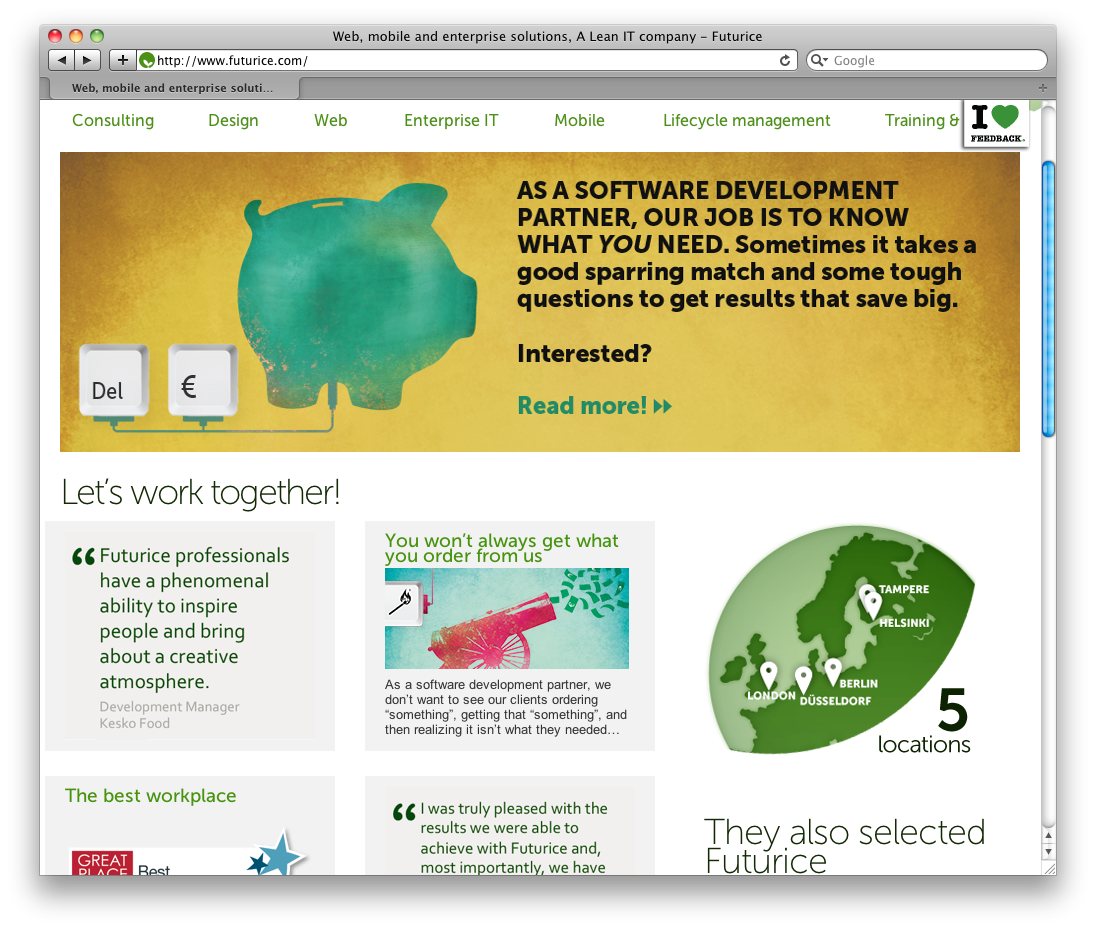
\includegraphics[width=1.0\textwidth]{initiate_feedback.png}
\end{center}
\caption{"I love feedback" button is added to the upper right corner of the website}
\end{figure}

When user presses the "I love feedback" button, a screen capture is taken from the website. After that, user is redirected to an editor, where user is able to draw on top of the captured website.

\subsubsection{Drawing tools}

In Hannotaatio, there are couple of tools for user to draw the feedback on top of the website. The number of tools have been kept minimum on purpose to make the application extremely simple to user.

The available drawing tools are pointing arrow, rectangle and text box. Also, the color of the drawing can be changes between dark and light color scheme. This allows user to draw on top of either light or dark websites.

In requirements gathering phase it was identified that the two most important functions of drawing tools are pointing, highlighting an area and leaving textual note. The three implemented drawing tools allow all the three. However, other drawing tools such as freehand drawing tool or circle drawing tool was left unimplemented, because they we're not critical tools to accomplish the desired functions of pointing, highlighting and leaving a note.

\begin{figure}[htb]
\begin{center}
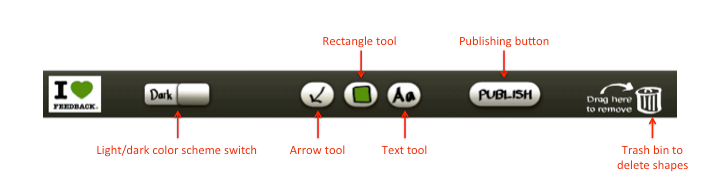
\includegraphics[width=1.0\textwidth]{drawing_tools_annotated_crop.png}
\end{center}
\caption{Hannotaatio toolbar}
\end{figure}

\subsubsection{Sharing the feedback with the team}

When the customer has drawn all the feedback with the available drawing tools, the first step to share the feedback with the team is to publish the feedback by pressing Publish button. When the drawn feedback is published no further modification can be made.

After publishing, user is given a secure URL, which she can share with the team for example via email. The secure URL is randomly generated UUID and it is long enough so that it is impossible to guess. That makes it secure even though viewing the feedback does not require password or any other user credential.

Optionally, if the team has set predefined notification email addresses, a notification email is sent to the team. This happens right after the feedback is published. If notification emails are used, customer does not have to share the secure URL with the team separately.

\subsubsection{Viewing the feedback}

After the drawn feedback has been published by the customer, the development team receives a notification email with the secure URL to the newly drawn feedback or the team receives the secure URL from the customer via email.

The team can now access to the published feedback. Besides seeing the drawn feedback the team can also see when the feedback was given and which browser and operation system was used. Additionally, team is able to access the original site from which the feedback was given by clicking "Go to original page". Also, team or whoever has access to the secure URL and delete the feedback by pressing "Delete" button.

\begin{figure}[htb]
\begin{center}
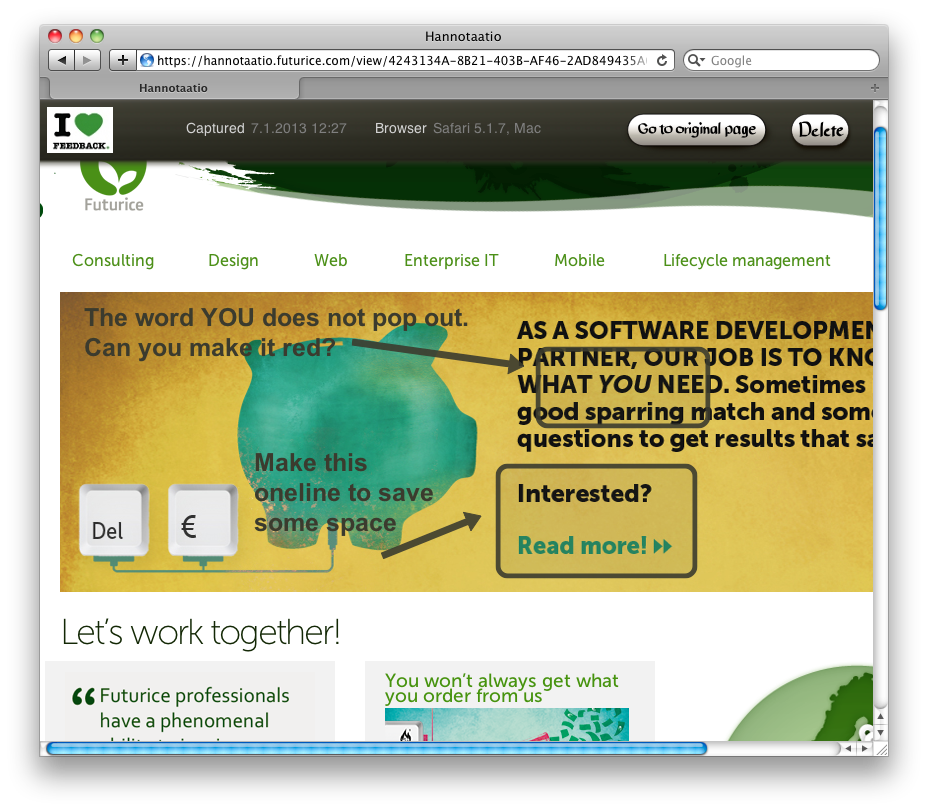
\includegraphics[width=1.0\textwidth]{published_feedback.png}
\end{center}
\caption{Published feedback}
\end{figure}

\subsection{Hannotaatio MRT}

Vastaa kysymykseen: Millainen kommunikaatiotyökalu Hannotaatio on MRT:n mukaan. Sopiiko palautteenantoon?

\subsection{Hannotaatio MST}

As noted in the previous sections, Media Synchronicity Theory identifies the following properties of a communication media: Transmission velocity, parallelism, natural symbol set, rehearsability and reprocessability.

In Hannotaatio the \textbf{transmission velocity} is low. When a developer team has something to show to the customer email is commonly used to notify customer about the new version from which she can give feedback. After the customer has received the notification from a developer team she browses to the site, gives feedback with Hannotaatio and shares the secure URL with the team via email.

The transmission speed of email is instant, but because getting a response to email adds some delay, email is considered to have low transmission velocity. Because there are at least two email send-receive cycles involved in one feedback which is given with Hannotaatio, it can be argued that the transmission velocity for Hannotaatio is rather low.

In Hannotaatio there is a possibility to use notification emails. If notification emails are used, the notification is sent to the team automatically right after the customer has published the feedback. This feature slightly improves the transmission speed because it eliminates one manual email sending from the whole feedback process.

Hannotaatio supports high \textbf{parallelism}. Because giving feedback with Hannotaatio does not require shared time and location with the feedback receiving team, customer can have many simultaneous feedback conversations at the same time. In the other words this means that customer can give feedback with Hannotaatio at the same time when shes chatting with the team with an instant messaging tool. However, it must be noted that drawing the feedback requires some concentration from the customer, so even if it is possible to have multiple conversions at the same time, it may not be very pleasent.

Hannotaatio supports also high \textbf{rehearsability}. Because the feedback is not transmitted to the developer team before customer chooses to publish it, customer has the ability to fine-tune the feedback drawing as long as she want. For feedback conversation this property of Hannotaatio is important, so that customer can fine-tune the message to be as clear and understandable as possible. Because feedback can be sometimes negative, it is also good that the customer has the ability to choose the wording carefully.

Hannotaatio supports high \textbf{reprocessability}. After the customer has shared the secure URL to the development team the team can come back to the URL which contains the message as many times as needed. From the feedback point-of-view this property of the tool is extremely important since the team may not have time to react to the feedback immediately. For example, in agile development, it might take some weeks before the team reacts to the feedback, it the team decides to do it in the next iteration. In this case it is important to be able to recap what was the feedback all about.

The naturalness of the \textbf{symbol set} in Hannotaatio can be argued to be medium. Visual message is more natural than for example written message. Because Hannotaatio supports visual encoding of the message (annotated screenshot) it has a more natural symbol set than e.g. plain text email, which (attachments excluded) supports only written message.

However, even though the message in Hannotaatio can be visually encoded, Hannotaatio misses for example vocal tones which can be transferred with for example telephone and physical gestures which can be transferred with for example video conferencing system or face-to-face. Thus it can be argued, that Hannotaatio does not have the most natural symbol set, instead medium level of naturalness.

\begin{table}[!h]
% increase table row spacing, adjust to taste
\renewcommand{\arraystretch}{1.3}
% if using array.sty, it might be a good idea to tweak the value of
% \extrarowheight as needed to properly center the text within the cells
\caption{Media capabilities and their importance for feedback}
\label{table:capabilities}
\centering
% Some packages, such as MDW tools, offer better commands for making tables
% than the plain LaTeX2e tabular which is used here.
\begin{tabular}{|p{4cm}|p{7cm}|p{3cm}|}
\hline
\textbf{Media \newline capability} & \textbf{Description} & \textbf{Support in Hannotaatio}\\
\hline
Transmission \newline velocity & The speed at which the information is transported from an individual to another & Low\\
\hline
Parallelism & Capability for multiple parallel communication sessions & High\\
\hline
Natural symbol set & Diversity of symbols which allows information encoding. Natural symbols are vocal tones and physical gestures etc. & Medium\\
\hline
Rehearsability & The ability to fine tune the message before sending it & High\\
\hline
Reprocessability & The possibility to reprocess the transmitted message & High\\
\hline
\end{tabular}
\end{table}

\subsection{Hannotaatio MNT}

Media Naturalness Theory emphasizes communication tools that are as natural as possbile, that is, as close to face-to-face communication as possible. The theory lists five key elements that involve in natural communication: high degree of co-location, high degree of synchronicity, ability to convey and observe body language and ability to convey and listen to speech.

Hannotaatio, as well as the other electronical communication media, does not support these properties well. Thus, from the Media Naturalness point-of-view, Hannotaatio is not very natural communication media. However, there are elements in Hannotaatio which make it superrior in comparison to other electronic communcation media, for example email.

The feedback in Hannotaatio is visual, which makes it more natural communication media than for example email of text-based chat rooms. However, Hannotaatio according to Media Naturalness Theory can not compete with for example video conferencing system, which has significantly better ability to convey the natural cues such as speech and body language.

However, \citep{kock2007} has suggested that managers should combine the media they are using. Hannotaatio is a combination of visual representation of the feedback and email notification, thus, according to Kock's prediction, the use of Hannotaatio should lead to reduction of text exchanged though email and thus lead to an overall increase in communication efficiency in communication.

In the future development of Hannotaatio, Media Naturalness Theory should be taken into more careful consideration. For example, there are improvement possibilities which would support Hannotaatio's naturalness. For example, instead of the static visual representation of the feedback the feedback could be recorded screen output of the user screen. In addition, an audio narration could be added. The audio narration would support Media Naturalness property listen to speech very well. In addition, a webcam video of the user itself could be included in order to capture the facial expressions and users body language. However, in the interviews many of the interviewee said that this would not add much value to the feedback and it would increase the barrier to give the feedback. Many of them said that they would feel themselves awkward if they would have to record their face while giving feedback. 

\begin{comment}
- Ehkä maininta "screencastista"
- Voiko tässä jo käyttää haastattelutuloksia? Kyl kai?
\end{comment}

\subsection{Hannotaatio MFT}
\label{sec:hannotaatio_mft}

In section~\ref{feedback_mft} the needs for feedback communication task were defined by the framework provided in the theory of Media Fitness \citep{higa2007}. In this section the mainly used communication tools, fax, telephone, email, instant messager, video conferencing system and face-to-face were used to evaluate their match to feedback communication task.

The feedback tool Hannotaatio can be evaluated by the same framework. As the needs of feedback communication task have been already defined in table~\ref{table:needs_for_feedback_communication_task} the same values can be used when evaluating Hannotaatio. The values of group I properties of Hannotaatio and the calculated match score are listed in table~\ref{table:hannotaatio_mft_scores}

\begin{table}[!h]
% increase table row spacing, adjust to taste
\renewcommand{\arraystretch}{1.3}
% if using array.sty, it might be a good idea to tweak the value of
% \extrarowheight as needed to properly center the text within the cells
\caption{Hannotaatio MFT scores}
\label{table:hannotaatio_mft_scores}
\centering
% Some packages, such as MDW tools, offer better commands for making tables
% than the plain LaTeX2e tabular which is used here.
\begin{tabular}{|p{3cm}|p{2cm}|p{2cm}|p{2cm}|p{2cm}|p{2cm}|}
\hline
\textbf{Property} & \textbf{Min} & \textbf{Best-} & \textbf{Best+} & \textbf{Max}\\
\hline
I-1 Response time & 1 & 1 & 3 & 4 \\
\hline
I-2 Security & 1 & 1 & 4 & 5 \\
\hline
I-3 Sharing & 4 & 4 & 5 & 5 \\
\hline
I-4 Retrieval & 1 & 1 & 2 & 3 \\
\hline
I-5 Multiparty & 1 & 1 & 3 & 4 \\
\hline
I-6 Expressive power & \multicolumn{4}{|p{10cm}|}{(1) Text: d (plain text), (2) Picture: ABC (digitalized, colored, high quality/resolution), (3) Voice: *, (4) Video: * } \\
\hline
\end{tabular}
\end{table}

By using the framework provided by the Media Fitness Theory, the media fit for group I properties to feedback communication task are: Response time: 1 (match), Security: 1 (match), Sharing: 1 (match), Retrieving: 0 (non-match), Multiparty: 1 (match). The total fit, which is the average of the match points gives total match of 0.667.

When the result is compared to the results of fitness of traditional communication media on table~\ref{group_i_match} it can be seen that Hannotaatio positioned to the second fittest medium after email (0.833) but before face-to-face (0.583). The closer look to the table reveals that properties of Hannotaatio are very close to properties of email. This is not a surprise, since Hannotaatio closely relies on email. The link to the given feedback is usually shared by notification emails or by manual email message from the feedback sender. From the match points between email and Hannotaatio it can be seen that Hannotaatio resulted with worse match points on retrieval. This is due the fact that Hannotaatio does not store the feedback URLs itself. The storing of the URL has to be done by feedback received herself.

\subsection{Hannotaatio, theoretical conclusion}

Edellisissä luvuissa käsiteltiin kutakin teoriaa ja Hannotaatiota erikseen. Tässä luvussa vedetään yhteen.

\subsection{Results of the semi-structured interviews}

Tässä luvussa kerrotaan haastattelujen tulokset.

\begin{itemize}
\item The interviews revealed that property A was very good
\item The interviews revealed that property B was missing and it would have been beneficial.
\end{itemize}


\begin{comment}
Tässä osassa esitetään tulokset ja vastataan tutkielman alussa
esitettyihin tutkimuskysymyksiin. Tieteellisen kirjoitelman
arvo mitataan tässä osassa esitettyjen tulosten perusteella. 

%% Huomaa seuraavassa kappaleessa lainausmerkkien ulkopuolella piste, 
%% koska piste ei lopeta lainattua tekstinpätkää.
%% Jos lainattu tekstinpätkä loppuu välimerkkiin, tulee välimerkki
%% lainausmerkkien sisälle: 
%% "Et tu, Brute?" sanoi Caesar kuollessaan.
Tutkimustuloksien merkitystä on aina syytä arvioida ja tarkastella
kriittisesti.  Joskus tarkastelu voi olla tässä osassa, mutta se
voidaan myös jättää viimeiseen osaan, jolloin viimeisen osan nimeksi
tulee >>Tarkastelu>>. Tutkimustulosten merkitystä voi arvioida myös
>>Johtopäätökset>>-otsikon alla viimeisessä osassa. 

Tässä osassa on syytä myös arvioida tutkimustulosten luotettavuutta.
Jos tutkimustulosten merkitystä arvioidaan >>Tarkastelu>>-osassa,
voi luotettavuuden arviointi olla myös siellä. 

\end{comment}

\clearpage

\section{Discussion}

\begin{enumerate}
\item What are the weak points of this study?
\item What could be studied in the future?
\end{enumerate}

\clearpage


\begin{comment}
Tässä osassa selvitetään, mitä tutkimuksen kohteena olevasta
aiheesta tiedetään entuudestaan. Selvityksen tulee kattaa
tasapainoisesti koko tutkimuskenttä. 

Kun opinnäytetyötä kirjoitetaan, on noudatettava 
ohjeita, jotka koskevat opinnäytteen rakennetta,
käytäntöjä, muotoseikkoja sekä ulkoasua. Esitellään näitä
ohjeita tarkemmin.
\end{comment}

%% Osan hienojaottelua alaosiin, eikä välttämättä edes tarpeen,
%% tässä vain esimerkkinä. Käytä harkintasi mukaan
%% osan jaottelua, joskus alaotsikot selventävät asioita ja
%% joskus vain sirpaloittavat tarpeettomasti tekstiä.
%%  Jaottelu menee seuraavasti:
%% \section{osan otsikko} 
%% \subsection{alaotsikko}
%% \subsubsection{ala-alaotsikko}
%% Tätä pitemälle ei pidä jaotella. 
%%
%% Three levels of hierarchy in sectioning should be enough

\begin{comment}
\subsection*{Rakenne}

Opinnäytteen rakenteen tulee olla hyvän tieteellisen
kirjoittamisen käytännön mukainen ja sisältää vähintään seuraavat
osat:

\begin{enumerate}
\item Nimiölehti
\item Tiivistelmä
\item Sisällysluettelo
\item Symboli- ja lyhenneluettelo
\item \label{a} Johdanto
%% Tässä alla on esimerkki lainausmerkkien käytöstä. Suomalaisen tekstin
%% lainausmerkit eivät mene oikein latexissa (tai monissa muissakaan
%% julkaisujärjestelmissä) kun käytetään
%% "-merkkiä, koska latex käyttää amerikkalaista lainausmerkkien
%% tulostustapaa. Vaihtoehtona voi käyttää kulmalainausmerkkejä, jotka
%% myös tulostuvat oikein.
\item  Aikaisempi tutkimus. Työn luonteen niin vaatiessa otsikko voi olla myös
        >>Teoreettinen tausta>>  tai näiden otsikoiden yhdistelmä.
\item Tutkimusaineisto ja -menetelmät %% yhdysmerkki - eli tavuviiva. 
\item Tulokset
\item \label{o} Tarkastelu. Työn luonteen niin vaatiessa otsikko voi
      olla myös >>Johtopäätökset>> tai >>Yhteenveto>> 
      tai edellä mainittujen otsikoiden yhdistelmä.
\item Lähteet
\item Liitteet.
\end{enumerate}

Tiivistelmän ja symboli- sekä lyhenneluetteloiden 
väliin voi sijoittaa halutessaan esipuheen.  

Työn osat \ref{a}-\ref{o} muodostavat \textit{tekstiosan.}  Työn
yksittäisiä osia voidaan jakaa alaotsikoilla alaosiin, joita ei ole
yllä esitetty. Alaotsikoiden käyttäminen selventää parhaimmillaan
tekstiä, ja pahimmillaan sirpaloittaa sitä.  Sirpaloitumista voi estää
huolehtimalla siitä, että samalla sivulla ei esiinny useampaa
alaotsikkoa.  Tekstin jäsentelyssä on yleensä ongelmia, jos osassa on
vain yksi alaosa, tai kirjoittaja joutuu käyttämään useampaa kuin
kahta tasoa (osa ja alaosat): alaosien alaosat ovat harvoin tarpeen.
\subsection*{Sivut ja kirjaintyypit}

Opinnäytteen tulee olla kirjoitettu koneella tai
tekstinkäsittelyohjelmalla yksipuolisesti A4-kokoiselle paperille.
Kandidaatintyön tekstiosan sopiva pituus on noin 15--20 sivua ja
diplomityön noin 60 sivua. Työtä ei ole syytä tarpeettomasti pidentää.

Opinnäytteen tekstiosan kirjaintyypin tulee olla antiikva eli
%% esimerkki pakkotavutuksesta; "serif-tyyppinen" on tavutuksen kannalta
%% hankala, joten pakkotavutetaan se. 
serif\--tyyp\-pi\-nen ja lisäksi kursivoimaton, lihavoimaton sekä kooltaan 12
pistettä (kuten tässä esityksessä). Groteskeja eli \textsf{Sans
  serif}-tyyppisiä kirjaintyyppejä (kuten Helvetica tai Arial) ei saa
käyttää varsinaisessa tekstissä, mutta otsikoissa näitä voidaan
käyttää.  Otsikoissa voidaan käyttää kooltaan edellä mainittua
suurempaa kirjaintyyppiä sekä tyylikeinoja, kuten lihavointia tai
kursivointia.  Tekstissä samantasoisten otsikoiden on kuitenkin oltava
tyyliltään ja kirjainlajeiltaan yhteneväisiä.
%% Esimerkki taulukosta
\begin{table}[htb]
%% Taulukon teksti
\caption{Taulukoissa ja kuvissa kirjaintyypin voi valita
tarkoituksenmukaisesti, mutta kuva- ja taulukkoteksteissä tulee
käyttää samaa kirjaintyyppiä kuin varsinaisessa tekstissä. 
Huomaa taulukon numeroinnin sijoittuminen taulukon yläpuolelle. \label{taulukko1}}
\begin{center}
\fbox{
\begin{tabular}{c|l|r}
\textbf{A} & 1 & $e^{j \omega t}$ \\ \hline
\textsf{B} & 2 & ${\mathfrak R}(c)$ \\ \hline
\texttt{C} & 3 & $ a \in \mathbb{A}$  
\end{tabular}
}
\end{center}
\end{table}

Opinnäytteen vasen marginaali (sidonnan puoli) on
35~mm % tässä ~ muodostaa ns. yhdistävän välilyönnin
ja oikea 25~mm. Ylämarginaali on 25~mm. Leipätekstin korkeus on
enimmillään 230mm. Tämän opinnäytepohjan marginaalien pitäisi olla
paperille tulostettuna oikein, mutta tulostimesta ja paperista
riippuen voi esiintyä yhden tai kahden millimetrin suuruisia eroja.
%% Jos käännät tämän tekstin pdflatex-komennolla ja tulostat sen katselu-
%% ohjelmasta, toteat todennäköisesti em. mittojen poikkeavan enemmän
%% kuin 1-2 mm. 
%% Tämä on seurausta pdf-tiedoston erilaisesta kirjaintyyppimäärityksestä.
%% Korkeatasoista painotyötä varten käytä vain latex-komentoa ja 
%% tulosta postscript-muotoon käännetystä tiedostosta. 
\subsection*{Asemointi}

%% Muutos vanhaan ohjeeseen verrattuna: aikaisemmassa ohjeessa
%% kehotettiin käyttämään vasensuora-asettelua, mutta tässä
%% ohjeessa ollaan luovuttu tuosta vaatimuksesta ja siirrytty
%% huoliteltumpaan, painotuotteenomaisempaan suuntaan.  
Tekstiosan tekstissä käytetään kappaleiden erottamiseen sisennystä,
mutta ensimmäistä otsikon, väliotsikon tai muun katkon jälkeistä
kappaletta ei sisennetä. Jos kuva tai muu katko tulee kappaleiden
väliin, suositellaan katkon jälkeisen kappaleen sisentämistä.

Mikäli oikea reuna halutaan tasata, tulee käyttää tavutusta ja lisäksi
tarkistaa, ettei tekstiin jää lukemista häiritseviä pitkiä sanavälejä. Jos
käytät opinnäytteen tekemisessä \LaTeX-järjestelmää, 
tämä asia hoituu automaattisest.

Opinnäytteen riviväli on 1, mikä on myös tämän opinnäytepohjan käytäntö. 
Kappaleiden tulee yleensä olla ainakin kolmen rivin pituisia, mutta
myös liian pitkiä kappaleita tulee välttää.  Tässä opinnäytepohjassa
ei tekstin luonteen vuoksi voida täysin toteuttaa kappaleen pituutta koskevia
vaatimuksia.

Yksittäisiä, kappaleen päättäviä tai aloittavia rivejä sivun alussa
tai lopussa on vältettävä koko työssä, myös luetteloissa ja
liitteissä.

\subsection*{Numerointi}

Opinnäytteen jokainen osa alkaa uudelta sivulta. Alaosa aloittaa uuden
sivun vain edellisen sivun täytyttyä.

Työn osat numeroidaan siten, että johdanto on ensimmäinen numeroitava
osa. Osien numeroinnissa käytetään arabialaisia numeroita.

Nimiölehti, tiivistelmä, esipuhe, sisällysluettelo ja symboli- ja
lyhenneluettelo numeroidaan esipuheesta tai tämän puuttuessa 
ensimmäiseltä luettelosivulta alkaen roomalaisin numeroin.

Sivunumerointi alkaa toiselta varsinaiselta tekstisivulta, ja 
sivunumeroinnissa käytetään arabialaisia numeroita.

Lähdeluettelo alkaa uudelta sivulta. Lähdeluettelon sivunumerointi 
jatkuu viimeisestä tekstisivusta.

Jokainen liite alkaa uudelta sivulta. Liitteiden sivunumerointi
jatkuu viimeisestä lähdeluettelon sivusta.

Sivunumero sijoitetaan sivun yläreunaan.

Matemaattiset kaavat numeroidaan arabialaisin
numeroin. Kaavanumerointi ei saa katketa osien välissä (eikä niin
tapahdukaan, jos käytät tätä opinnäytepohjaa). Kaikkia kaavoja ei tarvitse
numeroida, vaan kirjoittaja voi käyttää harkintaa numeroinnin
tarpeellisuudessa.  Liitteissä olevat kaavat numeroidaan siten, että
liitteen ajatellaan muodostavan numeroinnin kannalta itsenäisen ja
yhtenäisen kokonaisuuden. Kaavan numero sijoitetaan oikealle puolelle
alla olevan esimerkin mukaisesti
\begin{equation}
D(xy) = (Dx)y + x(Dy),  \hspace{3em} x,y \in \mathbb{A}.
\end{equation}
%% Kaavojen jälkeen ei yleensä laiteta sisennystä. 
Kaikki kuvat ja taulukot numeroidaan erillisen juoksevan numeroinnin
mukaisesti kuten taulukosta \ref{taulukko1} ja kuvasta \ref{kuva1} käy
ilmi.  Liitteissä olevat kuvat ja taulukot numeroidaan siten, että
liitteen ajatellaan muodostavan numeroinnin kannalta itsenäisen ja
yhtenäisen kokonaisuuden. Liitteissä \ref{LiiteA} ja \ref{LiiteB} on
esimerkkejä kaavojen (kaavat \ref{liitekaava1}--\ref{liitekaava2} tai
kaavat \ref{liitekaava3}--\ref{liitekaava4}), kuvien (kuva
\ref{liitekuva}) ja taulukoiden (taulukko \ref{liitetaulukko})
numeroimisesta.  Liitteet numeroidaan suuraakkosin (esimerkiksi Liite
A, Liite B tai pelkästään A, B).
%% Tässä esimerkki kuva1.pdf -nimisen tiedoston tuomisesta kuvaksi.
%% Komento \inclugraphics[parametrit]{argumentti} tuo kuvan.
%% Komento \centering pakottaa kuvan keskelle. 
%% Komento \caption luo kuvatekstin ja sen numeroinnin
%% Parametrit htb pakottavat kuvan suunnilleen siihen 
%% kohtaan, missä se esiintyy tekstin lähdekoodissa
\begin{figure}[htb]
\centering \includegraphics[height=5cm]{kuva1}
\caption{Tämä on esimerkki numeroidusta kuvatekstistä. \label{kuva1}}
\end{figure}

\subsection*{Lähdeviittausten käyttö} 

\begin{comment}

Lähdeviittaukset tulee tehdä huolellisesti ja johdonmukaisesti
numeroviitejärjestelmän mukaisesti. Numeroviitteet järjestetään
lähdeluetteloon viittausjärjestykseen, mutta jos lähdeluettelo
on hyvin laaja (useita sivuja), järjestetään viitteet pääsanan 
mukaiseen aakkosjärjestykseen. Alaviitejärjestelmää
\footnote{Myöskään alaviitteenä olevia kommentteja \underline{ei} suositella
käytettäviksi.} ei käytetä. 

Viitteen sijoittelussa noudatetaan seuraavia sääntöjä:
Jos viite kohdistuu vain yhteen virkkeeseen tai virkkeen 
osaan, viite \cite{Kauranen} sijoitetaan virkkeen sisään ennen virkettä
päättävää pistettä. Jos taas viite koskee tekstin useampaa
virkettä tai kokonaista kappaletta, sijoitetaan viite kappaleen loppuun 
pisteen jälkeen. \cite{Kauranen} 

\subsection*{Lähdeluettelo} 

Lähdeluettelossa esiintyy tavallisesti seuraavassa esitettäviä
lähteitä, joista on numeroviitejärjestelmässä ilmoitettava
asianomaisessa kohdassa vaaditut tiedot.

%% Esimerkki korostamisesta. Lihavoinnin sijasta on tyylikkäämpää
%% ja luettavampaa käyttää kursiivia.
\textit{Kirjasta} ilmoitetaan seuraavat tiedot:

\begin{itemize}
\item[--]tekijät 
\item[--]julkaisun nimi
\item[--]painos, jos useita
\item[--]kustannuspaikka
\item[--]julkaisija tai kustantaja
\item[--]julkaisuaika
\item[--]mahdollinen sarjamerkintö. 
\end{itemize}

Viitteet \cite{Kauranen}--\cite{Koblitz} ovat esimerkkejä kirjan
esittämisestä lähdeluettelossa. Viite \cite[s.\ 83--124]{Koblitz} on
esimerkki lähdeluettelossa esiintyvän kirjan tiettyjen sivujen
esittämisestä tekstissä.

\textit{Artikkelista} kausijulkaisussa ilmoitetaan seuraavat tiedot:

\begin{itemize}

\item[--]tekijät
\item[--]artikkelin nimi
\item[--]kausijulkaisun nimi
\item[--]julkaisuvuosi
\item[--]kausijulkaisun volyymi tai ilmestymisvuosi
\item[--]kausijulkaisun numero
\item[--]sivut, joilla artikkeli on.
\end{itemize}

Viitteet \cite{bcs}--\cite{Deschamps} ovat esimerkkejä artikkelin
esittämisestä lähdeluettelossa.

\textit{Kokoomateoksen luvusta tai osasta} ilmoitetaan seuraavat tiedot:

\begin{itemize}
\item[--]luvun tai osan tekijät
\item[--]luvun tai osan nimi
\item[--]maininta >>Teoksessa>>
\item[--]koko teoksen toimittajat sekä maininta >>(toim.)>>
\item[--]koko teoksen tai konferenssin nimi
\item[--]konferenssiesitelmän kyseessä ollessa sen pitopaikka ja -aika
\item[--]painos, jos useita
\item[--]kustannuspaikka
\item[--]julkaisija tai kustantaja, jos aihetta tämän ilmoittamiseen on
\item[--]julkaisuaika
\item[--]sivut, joilla luku tai osa on 
\item[--]mahdollinen sarjamerkintä.
\end{itemize}

Viitteet \cite{Sihvola}--\cite{Lindblom} ovat esimerkkejä
kokoomateoksen luvun tai osan esittämisestä lähdeluettelossa. 

\textit{Opinnäytetyöstä} ilmoitetaan seuraavat tiedot:

\begin{itemize}
\item[--]tekijä
\item[--]työn nimi
\item[--]opinnäytetyön tyyppi
\item[--]oppilaitoksen nimi
\item[--]osaston, laitoksen tai ohjelman nimi
\item[--]oppilaitoksen sijaintipaikka
\item[--]vuosiluku.
\end{itemize}

Viitteet \cite{Miinusmaa}--\cite{Lonnqvist} ovat esimerkkejä
opinnäytteen esittämisestä lähdeluettelossa. 

\textit{Standardista} ilmoitetaan seuraavat tiedot:

\begin{itemize}
\item[--]standardin tunnus ja numero
\item[--]standardin nimi
\item[--]painos, mikäli ei ole ensimmäinen
\item[--]julkaisupaikka
\item[--]julkaisija
\item[--]julkaisuvuosi
\item[--]sivumäärä.
\end{itemize}
Viite \cite{sfs} on esimerkki standardin esittämisestä opinnäytteen
lähdeluettelossa. 

\textit{Haastattelusta} ilmoitetaan seuraavat tiedot:

\begin{itemize}
\item[--]haastatellun henkilön nimi
\item[--]haastatellun henkilön arvo tai asema
\item[--]haastatellun henkilön edustama organisaatio
\item[--]organisaation osoite
\item[--]maininta siitä, että kyseessä on haastattelu ja haastattelun
päivämäärä. 
\end{itemize}

Viite \cite{haastattelu} on esimerkki 
haastattelun esittämisestä lähdeluettelossa.

Osa sähköisessä muodossa olevista artikkeleista on saatavissa myös
painettuina. \textit{Vain verkosta saatavissa olevasta artikkelista} esitetään
seuraavat tiedot:

\begin{itemize}
\item[--]tekijät
\item[--]artikkelin nimi
\item[--]kausijulkaisun nimi
\item[--]viestintyyppi
\item[--]laitos tai volyymi
\item[--]kausijulkaisun yksittäistä osaa koskeva merkintä tai numero
\item[--]julkaisuvuosi tai maininta >>Päivitetty>> ja päivitysaika
\item[--]maininta >>Viitattu>> ja viittaamisen ajankohta 
\item[--]maininta >>Saatavissa>> ja URL tai 
        maininta >>DOI>> ja DOI-numero (DOI=Digital Object Identifier).
\end{itemize}

Viitteet \cite{Ribeiro}--\cite{kone} ovat esimerkkejä sähköisessä
muodossa olevan artikkelin esittämisestä opinnäytteen
lähdeluettelossa.  Viitteet \cite{Ribeiro} ja \cite{Stieber} ovat
saatavissa sekä painettuna että verkosta, joten viitteiden esitystapa
mukailee painetun artikkelin viitteen esitystapaa, mutta sen lisäksi
kerrotaan julkaisun olevan verkkolehti ja lehden olevan saatavissa
myös painettuna.  Viite \cite{kone} on saatavissa vain verkosta ja
siitä esitetään yllä vaaditut tiedot.

Valitettavasti sähköisessä muodosssa olevasta artikkelista ei ole aina 
saatavissa lai\-tos-, volyymi- tai numerotietoja.

\textit{Sähköisessä muodossa olevasta opinnäytetyöstä} ilmoitetaan
seuraavat tiedot:
 
\begin{itemize}
\item[--]tekijä
\item[--]työn nimi
\item[--]viestintyyppi
\item[--]opinnäytetyön tyyppi
\item[--]oppilaitoksen nimi
\item[--]osaston, laitoksen tai ohjelman nimi
\item[--]oppilaitoksen sijaintipaikka
\item[--]vuosiluku
\item[--]viittamisen ajankohta
\item[--]maininta >>Saatavissa>> ja URL tai 
        maininta >>DOI>> ja DOI-numero.
\end{itemize}

Viite \cite{Adida} on esimerkki sähköisessä muodossa olevan
opinnäytteen esittämisestä lähdeluettelossa.

Viite \cite{viittaaminen} on esimerkki itsenäisen kirjoituksen sisältävästä
verkkosivusta. Tällainen lähde on rinnastettavissa erillisteokseen.
\textit{Verkkosivusta} esitetään tiedot:

\begin{itemize}
\item[--] tekijät
\item[--] otsikko
\item[--] maininta >>Päivitetty>> ja päivitysaika 
\item[--] maininta >>Viitattu>> ja viittaamisen ajankohta
\item[--] Maininta >>Saatavissa>> ja URL.
\end{itemize}

Joskus verkkosivun kirjoitus on jaettu useammalle sivulle, jolloin
lähdeluetteloon kirjataan vain sellainen verkko-osoite, joka koskee
koko kirjoitusta tai sen etusivua, ellei sitten 
todella tarkoiteta kirjoituksen yksittäistä sivua. 

\subsection*{Muuta huomioitavaa lähdeluettelossa}

%% Muutos vanhoihin ohjeisiin koskien kieltä.
Lähdeluettelossa työn ja julkaisun nimi kirjoitetaan alkuperäisessä
muodossaan. Julkaisijan kotipaikka kirjoitetaan alkukielisessä
muodossaan.

Viittamista koskevassa suomalaisessa standardissa
SFS 5342 \cite{sfs} vaaditaan julkaisuista ilmoitettavaksi myös ISBN- tai
ISSN-numerot, mutta näissä opinnäyteohjeissa ei ISBN- ja 
ISSN-numeroita vaadita. 

\end{comment}

%% Lähdeluettelo
\bibliographystyle{plainnat}
\bibliography{ref}


%% Liitteet 
\appendix 

\clearpage

% \addcontentsline{toc}{section}{Appendix A}
\section{Interview Questions\label{appendix:interview_questions}}

Alustus: Teen haastattelun diplomityötäni varten Aalto-yliopiston informaatioverkostojen koulutusohjelmaan. Haastattelulla pyrin selvittämään Hannotaatio palautetyökalun käyttöä sekä palautteen antamista yleisemmin ohjelmistoprojekteissa. Haastattelu nauhoitetaan. 

\begin{enumerate}

\item Titteli, ikä? Saanko käyttää näitä työssäni?

\item Yritys, jossa työskentelet? Saanko tarvittaessa käyttää näitä työssäni?

\item Kerrotko lyhyesti, mitä sinä ja yrityksesi teette?

\item Miten yrityksessänne hoidetaan palautteen anto asiakas-toimittaja suhteessa?

\item Mitkä asiat vaikuttavat siihen, millä tavoin ja millä välineillä palautekommunikaatio hoidetaan?

\item Millaisessa projektissa olette käyttäneet Hannotaatiota?

\item Miten Hannotaation käyttö on muuttanut palautteenantoa, vai onko?
  \begin{enumerate}
    \item Miten paljon palautetta on tullut Hannotaation kautta?
    \item Miksi niin paljon / miksi niin vähän?
  \end{enumerate}


\item Miten paljon arvostat palauttetyökalussa seuraavia ominaisuuksia:
  \begin{enumerate}
    \item Palautteen antamisen / saamisen jälkeen keskusteluyhteyden on jatkuttava samantien (esim. tarkentavat kysymykset) \textit{Välitön palaute / vastausaika (MRT, MST, MFT)}
    
    \item Persoonallisuus, eli palauttessa pitää näkyä ja tuntua oman kädenjälkesi \textit{Persoonallisuus (MRT)}
    
    \item Mahdollisuus ilmaista palaute mahdollisimman monilla tavoilla, esimerkiksi tekstillä, kuvilla, äänellä, videolla, eleille, äänenpainolla? \textit{Ilmaisun monimuotoisuus (MRT, MST, MFT)}
    
    \item Mahdollisuus ilmaista palaute ihmiselle luonnollisilla ilmaisutavoilla (esim kuva vs. teksti, video vs. ääni) \textit{Ilmaisun luonnollisuus (MRT, MST, MFT)}
    
    \item Mahdollisuus olla samanaikaisesti mukana useammassa kommunikaatiotilanteessa (esim face-to-face vs. IM) \textit{Samanaikaisuus (MST)}
    
    \item Mahdollisuus muokata, editoida ja viimeistellä palautetta ennen lähettämistä \textit{Mahdollisuus viimeistellä (MST)}
    
    \item Mahdollisuus palata annettuun palautteeseen ja tulkita se uudelleen \textit{Mahdollisuus uudelleenprosessointiin (MST)}
    
    \item Turvallisuus, tietojen pysyminen vain halutuilla kommunikaatiotahoilla \textit{Turvallisuus (MFT)}
    
    \item Helppo jaettavuus muille kuin kommunikaatiotapahtumasa mukana olleille \textit{Helppo jaettavuus (MFT)}
    
    \item Mahdollisuus indeksoida palaute myöhempää hakua varten \textit{Haku myöhempää käyttöä varten (MFT)}
    
    \item Mahdollisuus monen käyttäjän yhteiskäyttöön (esim. Google Docs) \textit{Monen käyttäjän yhtäaikainen käyttö (MFT)}
    
    \item Mahdollisuus antaa palautetta ajallisesti milloin vain (ei pelkästään työaikana) \textit{Saavutettavuus ajallisesti (MFT)}
    
    \item Mahdollisuus antaa palautetta sijainnillisesti mistä vain (ei pelkästään toimistosta) \textit{Saavutettavuus fyysisesti (MFT)}
    
    \item Kommunikaatiotyökalun käytön kustannukset \textit{Hinta (MFT)}
    
  \end{enumerate}
  
\item Miten nämä ko. ominaisuudet on toteutettu mielestäsi Hannotaatiossa?
  
\item Millaisia uusia ominaisuuksia kaipaisit Hannotaatioon (jotta siitä tulisi entistä parempi työkalu palautteenantoon)? \textit{MNT}
  \begin{enumerate}
    \item Videokuva palautteen piirtämisestä?
    \item Videokuva + ääniraita
    \item Videokuva + ääniraita + videokuva palautteenantajasta
  \end{enumerate}

\item Onko sinulla vielä jotain muuta jota haluaisit lisätä koskien palautteen antoa yleisesti tai Hannotaatio-työkalua?
  
\end{enumerate}

\clearpage

\begin{comment}
\addcontentsline{toc}{section}{Liite A}
\section{Esimerkki liitteestä\label{LiiteA}}
%% Liitteiden kaavat, taulukot ja kuvat numeroidaan omana kokonaisuutenaan
%%
%% Equations, tables and figures have their own numbering in Appendices
\renewcommand{\theequation}{A\arabic{equation}}
\setcounter{equation}{0}  
\renewcommand{\thefigure}{A\arabic{figure}}
\setcounter{figure}{0}
\renewcommand{\thetable}{A\arabic{table}}
\setcounter{table}{0}

Liitteet eivät ole opinnäytteen kannalta välttämättömiä ja 
opinnäytteen tekijän on 
kirjoittamaan ryhtyessään hyvä ajatella pärjäävänsä ilman liitteitä.
Kokemattomat kirjoittajat, jotka ovat huolissaan
tekstiosan pituudesta, paisuttavat turhan 
helposti liitteitä pitääkseen tekstiosan pituuden annetuissa rajoissa.
Tällä tavalla ei synny hyvää opinnäytettä.   

Liite on itsenäinen kokonaisuus, vaikka se täydentääkin tekstiosaa.
Liite ei siten ole pelkkä listaus, kuva tai taulukko, vaan 
liitteessä selitetään aina sisällön laatu ja tarkoitus. 

Liitteeseen voi laittaa esimerkiksi listauksia. Alla on 
listausesimerkki tämän liitteen luomisesta. 

%% Verbatim-ympäristö ei muotoile tai tavuta tekstiä. Fontti on monospace.
%% Verbatim-ympäristön sisällä annettuja komentoja ei LaTeX käsittele. 
%% Vasta \end{verbatim}-komennon jälkeen jatketaan käsittelyä.
\begin{verbatim}
    \clearpage
	\appendix
	\addcontentsline{toc}{section}{Liite A}
	\section*{Liite A}
	...
	\thispagestyle{empty}
	...
	tekstiä
	...
	\clearpage
\end{verbatim}

Kaavojen numerointi muodostaa liitteissä oman kokonaisuutensa:
\begin{eqnarray}
d \wedge A  &=& F, \label{liitekaava1}\\
d \wedge F  &=& 0. \label{liitekaava2}
\end{eqnarray}


\clearpage
\addcontentsline{toc}{section}{Liite B}
\section{Toinen esimerkki liitteestä\label{LiiteB}}

%% Liitteiden kaavat, taulukot ja kuvat numeroidaan omana kokonaisuutenaan
%%
%% Equations, tables and figures have their own numbering in Appendices
\renewcommand{\theequation}{B\arabic{equation}}
\setcounter{equation}{0}  
\renewcommand{\thefigure}{B\arabic{figure}}
\setcounter{figure}{0}
\renewcommand{\thetable}{B\arabic{table}}
\setcounter{table}{0}

Liitteissä voi myös olla kuvia, jotka
eivät sovi leipätekstin joukkoon:
%% Ympäristön figure parametrit htb pakottavat
%% kuvan tähän, eikä LaTeX yritä siirrellä niitä
%% hyväksi katsomaansa paikkaan. 
%% Ympäristöä center voi käyttää \centering-
%% komennon sijaan
%%
%% Example of a figure, note the use of htb parameters which force
%% the figure to be inserted here
\begin{figure}[htb]
\begin{center}
\includegraphics[height=8cm]{kuva2}
\end{center}
\caption{Kuvateksti, jossa on liitteen numerointi \label{liitekuva}}
\end{figure}
%%
Liitteiden taulukoiden numerointi on kuvien ja kaavojen kaltainen:
\begin{table}[htb]
\caption{Taulukon kuvateksti. \label{liitetaulukko}}
\begin{center}
\fbox{
\begin{tabular}{lp{0.5\linewidth}}
9.00--9.55  & Käytettävyystestauksen tiedotustilaisuus (osanottajat
ovat saaneet sähköpostitse valmistautumistehtävät, joten tiedotustilaisuus
voidaan pitää lyhyenä).\\
9.55--10.00 & Testausalueelle siirtyminen
\end{tabular}}
\end{center}
\end{table}
Kaavojen numerointi muodostaa liitteissä oman kokonaisuutensa:
\begin{eqnarray}
T_{ik} &=& -p g_{ik} + w u_i u_k + \tau_{ik},  \label{liitekaava3} \\
n_i    &=& n u_i + v_i.                        \label{liitekaava4}
\end{eqnarray}

\end{comment}

\end{document}